%%%%%%%%%%%%%%%%%%%%%%%%%%%%%%%%%%%%%%%%%
% Template for CWRU CDS Qualify Exam
% Version 1.0 (10-Jul-2023)
%
% Original author:
% Mengying Wang
%%%%%%%%%%%%%%%%%%%%%%%%%%%%%%%%%%%%%%%%%

% QE written report requirements of the CDS department: 11 pt font, single-spaced, single column, 1" margins.

% Fill in your title, name, and committee members in commands.tex.

\documentclass[11pt, letterpaper]{article}

% Load necessary packages
\usepackage[utf8]{inputenc}
\usepackage[T1]{fontenc}
\usepackage[english]{babel}
\usepackage{amsmath,amssymb,amsfonts}
\usepackage{graphicx}
\usepackage{float}
\usepackage{setspace}
\usepackage{xspace}
\usepackage{lipsum} % For generating dummy text. 
\usepackage[margin=1in]{geometry}
\usepackage{titlesec} % For customizing section titles
\usepackage{abstract} % For customizing abstract
\usepackage[round,sort&compress]{natbib}
%\usepackage[round,sort&compress,sectionbib,authoryear]{natbib}% For bibliography
%\bibliographystyle{abbrvnat} 
\bibliographystyle{aasjournal}
%\bibliographystyle{apj}
\usepackage{hyperref}
\hypersetup{
    colorlinks=true,
    citecolor=blue,
    filecolor=blue,
    linkcolor=blue,
    urlcolor=teal
}



\usepackage{multibib}
\usepackage{tcolorbox}

\newcites{mypub}{Published}
\newcites{review}{Under Review}
\newcites{prepare}{In Preparation}


\singlespacing % Set single spacing
\setlength{\parskip}{0.25\baselineskip} % Set paragraph spacing

% \input{commands}

% Meta Information
\newcommand{\qetitle}{The cosmic dance of galaxies and their Massive black holes}
\newcommand{\name}{Pranav Satheesh}
\newcommand{\degreeaward}{Ph.D. in Physics} 
\newcommand{\department}{Department of Physics} 
\newcommand{\university}{University of Florida} 
\newcommand{\monthyeardate}{\ifcase \month \or January\or February\or March\or April\or May\or June\or July\or August\or September\or October\or November\or December\fi, \number \year}
% \newcommand{\monthyeardate}{June, 2023}

% Committee Members
\newcommand{\chair}{Your Chair}
\newcommand{\advisor}{Your Advisor}
\newcommand{\committee}{Committee Member}



%equations
\newcommand{\msun}{M$_{\odot}$}
\newcommand{\msunyr}{M$_{\odot}$ yr$^{-1}$}
\newcommand{\kms}{km s$^{-1}$}
\newcommand{\inv}{$^{-1}$}
\newcommand{\vk}{$v_{\rm k}$}
\newcommand{\vesc}{$v_{\rm esc}$}
\newcommand{\tmrg}{$t_{\rm mrg}$}
\newcommand{\tcoal}{$t_{\rm coal}$}
\newcommand{\fgas}{$f_{\rm gas}$}
\newcommand{\tagn}{$t_{\rm AGN}$}
\newcommand{\tobs}{$t_{\rm obs}$}
\newcommand{\hbeta}{H{$\beta$}}
\newcommand{\oiii}{[O{\rm\,III}]}
\newcommand{\lhbeta}{$L_{\rm H\beta}$}
\newcommand{\lbol}{$L_{\rm bol}$}
\newcommand{\SB}{\textcolor{red}{SB23}}
\newcommand{\qin}{$q_{\rm in}$}
\newcommand{\qout}{$q_{\rm out}$}


\newcommand{\ps}[1]{{\bf\textcolor{red}{{#1}}}}


\begin{document}

\pagenumbering{roman}

% Title page
\begin{titlepage}
    \begin{center}
        \vspace*{0.3in}
        \Huge{\textbf{\MakeUppercase{\qetitle}}}

        \vspace{0.35in}
        \Large{\textbf{by}}
        
        \vspace{0.45in}
        \Large{\textbf{\MakeUppercase{\name}}}
        
        \vspace{0.5in}
        \Large{A qualifying examination submitted in partial fulfillment \\
        of the requirements for the degree of \\
        \degreeaward}

        \vspace{0.8in}
        \large{Committee Members: \\
        Dr. Laura Blecha (Chair)\\
        Dr. Jeff Andrews \\
        Dr. Siyao Xu \\
        Dr. Anthony Gonzalez}
 

        \vspace{0.7in}
        \Large{\department \\
        \university \\
        \monthyeardate}
    \end{center}
\end{titlepage}


% % Abstract page
% \thispagestyle{plain}
% \begin{center}
%     \Large
%     \textbf{\qetitle}
        
%     \vspace{0.13in}
%     \textbf{\name}
    
%     \vspace{0.13in}
%     \normalsize{Committee: Dr. \chair(Chair), Dr. \advisor(Advisor), Dr. \committee}
       
%     \vspace{0.3in}
%     \large
%     \textbf{Abstract}
% \end{center}
% % Add your abstract here
\lipsum[1]

% Keywords
\noindent \textbf{Keywords:} keyword1, keyword2, keyword3
% \newpage


% Table of contents
\tableofcontents
\newpage

\pagenumbering{arabic}

\section{Motivation}

Massive black holes (MBHs) are found in the centers of most massive galaxies \citep{Kormendy_1995,magorrian_demography_1998} and play a key role in galaxy evolution, as evidenced by the correlation between MBH masses and stellar bulge properties \citep{ferrarese_fundamental_2000,gultekin_m-sigma_2009,Kormendy_2013,mcconnell_revisiting_2013}. Such correlations in the local universe imply the co-evolution between host galaxies and their central black holes (BHs). During galaxy mergers, gravitational interactions extract angular momentum from gas and funnel it toward the galactic center, triggering bursts of star formation and episodes of high accretion on to the central MBH \citep{Barnes_and_Hernquist_1992}. Such 
accreting BHs or Active Galactic Nuclei (AGN) are responsible for regulating star formation in massive galaxies at low redshift via feedback process \citep{DiMatteo_2005,Vogelsberg_2014a}. 



Despite their importance, however, the formation and early evolution of massive black holes remain poorly understood. Current formation models propose that MBH ``seeds" form early in the Universe via one or more mechanisms \citep{Madau_2001,Davies2011,Bromm_Loeb_2003} and grow across cosmic time via gas accretion and mergers. In the hierarchical model of structure formation, galaxy mergers drive MBH mergers — a process spanning vast spatial scales \citep{Begelman1980,merritt_massive_2005}, from kpc separations during galaxy mergers to sub-pc in the final stages of black hole (BH) coalescence (see Figure \ref{fig:path-to-merger}). The efficiency of MBH binary hardening depends on the properties of the host environment, and it is not assured that the MBHs will merge within a Hubble time \citep{2003MerritandMilosavljevic}. 

MBH binaries (MBHBs) are the loudest gravitational wave (GW) sources in the universe, with chirp frequencies ranging from millihertz (mHz) for MBHs around $\sim 10^6$ \msun{} to nanohertz (nHz) for MBHs around $10^8$ \msun{} \citep{Sesana2013}. In the nanohertz frequency range, GWs from a population of MBHBs can combine to produce a gravitational wave background (GWB). Pulsar timing arrays (PTAs) around the world have found compelling evidence for a GWB that is consistent with a MBHB origin of the background \citep{agazie_nanograv_2023,antoniadis_second_2023,reardon_search_2023,xu_searching_2023}. The early growth and evolution of MBHs will be directly probed by the planned Laser Interferometer Space Antenna (LISA), which will detect gravitational waves (GWs) from merging binaries with masses in the range $\sim 10^3$ - $10^7$ \msun{} out to redshifts of $z \sim 20$ \citep{Amaro2017lisa}. The merger rates of MBHs observed by LISA will be sensitive to MBH formation mechanisms and merger timescales. Current predictions of these rates vary significantly, with estimates ranging from a few to tens of detections per year, depending on the assumptions and physics included in the models \citep{Klein_2016,Kelley_2017a,Kelley_2018,Dayal_2019,Katz2020}. This uncertainty highlights the need for improved modeling tools that incorporate relevant physics to study how MBH formation mechanisms, dynamics, and growth collectively shape merger rates. 

Electromagnetic (EM) observations from missions such as the James Webb Space Telescope (JWST) will complement LISA's GW observations by exploring MBH origins and assembly in the early Universe. JWST has already begun transforming our understanding of the high-redshift Universe with detections of several Active Galactic Nuclei (AGN) between $z \sim 4-11$ that are $\sim 10-100$ times more massive than expected by local BH-galaxy scaling relations \citep{Larson_2023, harikane2023jwstnirspeccensusbroadlineagns, matthee2024littlereddotsabundant, goulding2023uncovergrowthmassiveblack}. These ``overmassive" BHs pose a challenge to existing MBH seed and growth models, with some studies \citep{Pacucci_2023,natarajan2023detectionovermassiveblackhole} suggesting they may require heavy seed scenarios — such as rapid collapse of massive gas clouds. To resolve these puzzles, theoretical studies of MBH populations must rigorously compare predictions with JWST observations.


Cosmological hydrodynamical simulations are powerful tools for studying the formation and evolution of MBH populations \citep{HorizonAGN2014,2015Illustris,2015Eagle,nelson2021illustristngsimulationspublicdata}. Although semi-analytical models \citep{Sesana_2011,Barausse_2012, Klein_2016,Dayal_2019,bonetti_post-newtonian_2019, Valiante_2020} offer a computationally inexpensive alternative, they cannot trace the internal structure and evolution of galaxies, which is a significant limitation
for modeling MBH binaries (MBHBs). In contrast, cosmological simulations self-consistently track the evolution of dark matter and baryons over large volumes.  However, there is an inherent trade-off between the size of the simulation and the mass and spatial resolution required to resolve MBHB dynamics. To address this, sub-grid models for MBH dynamics are required to account for hardening processes that shrink the MBHB orbit till their merger. Semi-analytic MBHB evolution models are used to compute merger timescales in post-processing of these cosmological simulations. 


A variety of physical effects — such as dynamical friction, stellar scattering, gas dynamics, triple interactions and GW emission, can affect binary hardening depending on the merging environment and must be accounted for when calculating merger timescales. After a merger, GW recoil kick imparted to the merger remnant by asymmetric GW emission \citep{Bekenstein1973} is another key dynamical effect. A BH subjected to GW recoil can exceed the host galaxy’s escape velocity and be ejected, which prevents subsequent mergers \citep{volonteri_gravitational_2007,Gerosa_2014,Blecha2016,sayeb_massive_2021}. Similarly, triple MBH interactions can also cause the ejection of the lightest MBH in the system via gravitational slingshot kicks \citep{volonteri_assembly_2003}. \textbf{Part of the goal of my work is to model MBH dynamics within these cosmological simulations and understand how the inclusion of different physical processes impacts MBH evolution.}

The MBH binary dynamics is heavily dependent on the host galaxy environment such as the host galaxy density and velocity profiles. Similarly, EM predictions depend on BH accretion rates which in turn depend on the local gas content. We have less understanding of the type of galaxies that host GW sources of merging MBHs which is required for us to pin down possible EM counterparts to future PTA and LISA detections. As cosmological simulations help us model the internal structure of these galaxies, we can study the host environment and their dependence on MBH formation and dynamics. At higher redshifts, BHs and galaxies retain signatures of their origins before subsequent accretion and merger events erase this information. Therefore a theoretical understanding of the host galaxy environment of the MBH mergers could give help us understand the BH-galaxy connection in the early universe better. At lower redshifts, these simulations can be used to create a mock sample of host galaxies of GW sources. \textbf{Characterizing the host galaxies of inspiralling and merging MBHs is another major goal of my proposed research}.

The following report is organized as follows. In Section \ref{sec:background}, I provide the necessary background for my work, including a description of the cosmological simulation suite used, the physics of MBH binary hardening, triple MBH interactions, BH kicks, and the properties of host galaxies of MBH binaries. In Section \ref{sec:MBH-dynamics-project}, I discuss the first topic of my proposed thesis: modeling the dynamics of MBHs in cosmological simulations. I also summarize the results from my previous work in this area and outline future research works. In Section \ref{sec:host-galaxy-project}, I explore the second topic: characterizing the host galaxies of MBH binaries. I present some preliminary results and discuss planned work. Finally, Section \ref{sec:timeline} provides a rough timeline of the planned activities for this project.


\section{Background}
\label{sec:background}

\subsection{Cosmological simulations}
\label{sec:cosmo-sim}

My work utilizes a suite of cosmological simulations, mainly the Illustris \citep{Vogelsberg_2014a,2015Illustris,Nelson_2015}, Illustris-TNG \citep{nelson2021illustristngsimulationspublicdata} and the BRAHMA simulations \citep{bhowmick2024introducingbrahmasimulationsuite,bhowmick2024growthhighredshiftsupermassive}. The Illustris simulation suite is a set of cosmological, hydrodynamical simulations run using the {\tt AREPO}  code \citep{Springel_2010}. This code combines the advantages of smooth particle (SPH) (e.g. \citep{Gingold_1977}) and an Eulerian-mesh-based approach (e.g. \citep{Berger_1989}). The highest resolution run, `Illustris-1'(referred to as Illustris), is a cosmological box of side $L_{\text{box}} = 75 h^{-1}$ Mpc. This simulation has a DM resolution of $6.3 \times 10^6 M_{\odot}$ and a baryonic mass resolution of $1,2 \times 10^6 M_{\odot}$ and runs from $z=137$ to $z=0$. The simulations assume a WMPA9 cosmology \citep{Hinshaw_2013} with parameters $\Omega_m = 0.2865$, $\Omega_{\Lambda} = 0.7135, \sigma_{8} = 0.820$, and $H_{0} = 70.4$ \kms Mpc$^{-1}$. 

Illustris also uses sub-grid models of stellar evolution, chemical enrichment, gas cooling, feedback from accreting MBHs and superovae \citep{Vogelsberger_2013,Torrey_2014}. BH particles are seeded with an initial mass of $1.4 \times 10^{5}$ \msun{} in halos of mass above $7.1 \times 10^{10}$ \msun{} that do not already contain an MBH \citep{2015Illustris}. The MBHs grow through Eddington-limited Bondi accretion and mergers \citep{Springel_2005,DiMatteo_2005}. The Eddington-limited Bondi-Hoyle formalism given by

\begin{align}
    \dot{M}_{\rm bh} &= \min \left( \dot{M}_{\rm bondi}, \dot{M}_{\rm Edd} \right) \\
    \dot{M}_{\rm bondi} &= \frac{4 \pi G^2 M^2_{\rm bh} \rho }{c^3_s}\\
    \dot{M}_{\rm Edd} &= \frac{4 \pi G M_{\rm bh} m_p }{\epsilon_r \sigma_T c}
\end{align}

where $G$ is the gravitational constant, $\rho$ is the local gas density, $M_{\rm bh}$ is the BH mass, $c_s$ is the local sound speed, $m_p$ is the proton mass, and $\sigma_T$ is the Thompson scattering cross section. Galaxies are identified by the Subfind algorithm \citep{Dolag_2009}, which located gravitationally bound “sub-halos” within friends-of-friends halos. The term “MBH host galaxies” used hereafter refer to the Subfind subhalos that host MBHs.

The next generation of Illustris simulation, called Illustris TNG has significant improvements over Illustris. The major improvement is a two-mode AGN feedback model.  sddd  For accretion rates that exceeds a critical, BH-mass-dependent fraction of the Eddington limit ($\eta_{\rm crit} = \min[0.002 (M_{\rm bh}/10^8 M_{\odot})^2,  0.1]$) thermal AGN feedback dominates where a part of the accreted mass energy is imparted to the surrounding gas as thermal energy. For accretion rates lower than this value, the AGN feedback is driven by winds, where kinetic energy is ejected into the surrounding gas at irregular intervals, in randomly chosen directions \citep{Weinberger_2016}. 

The fiducial IllustrisTNG box volume is $(100 \, \rm Mpc)^3$,
but it also features both higher-resolution $(50 \, \rm Mpc)^3$
and lower-resolution $(300 \, \rm Mpc)^3$volumes. Like most large-volume cosmological simulations TNG simply seed $8 \times 10^{5} M_{\odot}/h$ BHs are seeded in $ > 5 \times 10^{10} M_{\odot}/h$
halos that do not already have a BH. Such simulations with limited gas mass resolution fail to capture the evolution of lower-mass MBHs ($\sim 10^3 - 10^4$ \msun{}) detectable by LISA. However, the recent BRAHMA simulations introduced novel sub-grid seeding methods in cosmological simulations, enabling seed masses as low as $\sim 10^3$ \msun{} and exploring both light and heavy seed formation scenarios \citep{bhowmick2023representinglowmassblack,bhowmick2024introducingbrahmasimulationsuite,bhowmick2024growthhighredshiftsupermassive,bhowmick2024signaturesblackholeseeding}. 

The BRAHMA simulations were run using the AREPO gravity + moving-mesh magnetohydrodynamics (MHD) code \citep{Springel_2010,Pakmor_2016,Weinberger_2020} and adopts most of the sub-grid recipes from the TNG simulations, with the exception of BH seeding. The primary simulations comprise of a series of boxes with volumes $(9 \, \rm Mpc)^3$, $(18 \, \rm Mpc)^3$ and $(36 \, \rm Mpc)^3$. The smallest volume box is capable of directly resolving $\sim 10^3 M_{\odot}$ mass seeds. In the higher volume boxes, the descendants of these seeds are seeded at their respective gas mass resolutions using a stochastic seeding model. These primary set of boxes are run until z = 7 and will be helpful in probing the population of low mass MBHs or intermediate mass black holes (IMBHs). 

There are several proposed scenarios for the formation of the first seeds of massive black holes. The light seed models include BH seeds with masses $\sim 10^2-10^3$ \msun{} from pop III stellar remnants \citep{Fryer_2001,Madau_2001,Smith_2018,Xu_2013} and remnants from runaway collisions in nuclear star clusters with masses of $10^3-10^4$ \msun{} \citep{Davis_1985,Lupi_2014,Kroupa_2020,Das_2021}. The heavy seed models are from direct collapse black holes and masses range from $\sim 10^4 -10^6$ \msun{} \citep{Bromm_Loeb_2003,Begelman_2006,Regan_2014}. Note that BRAHMA simulations doesn't explicitly resolve the $\sim 10^2$ \msun{} as that would be computationally expensive. Instead, the smallest resolution volume box resolve a target seed mass of $2.3 \times 10^{3}$ \msun{}. These could thus represent either the most massive pop-III seeds or the low mass NSC seeds. These are referred to as "direct gas based" seeds or DGBs and are placed in halos with a minimum threshold of dense and metal poor (star-forming) pristine gas. The halos should also exceed a critical mass threshold. 

Although the DGBs form in halos that are biased to lower metallicities, it is seen that their higher mass descendants end up with unbiased galaxies, characterized totally by their total galaxy mass \citep{bhowmick2023representinglowmassblack}. The descendants of the DGBs in the $(18 \, \rm Mpc)^3$ and $(36 \, \rm Mpc)^3$ boxes are called the “extrapolated seed descendants” or ESDs. ESDs are then stochastically placed in galaxies that exceed a threshold mass which are drawn from galaxy mass distributions of wherein the $2.3 \times 10^{3}$ \msun{} DGBs end up within the $(9 \, \rm Mpc)^3$  simulation. Thus, the seeding in these simulations can be described by two criteria: i) dense and metal poor gas mass and ii) halo mass criteria. The halos must have a critical threshold in the gas mass that is dense enough to form stars ($n_H \gtrsim 0.1 \rm cm^{-3} $), metal poor ($Z < 10^{-4} \, Z_{\odot}$) and are above a minimum threshold in their total mass. 

\begin{figure}[!htb]
    \centering
    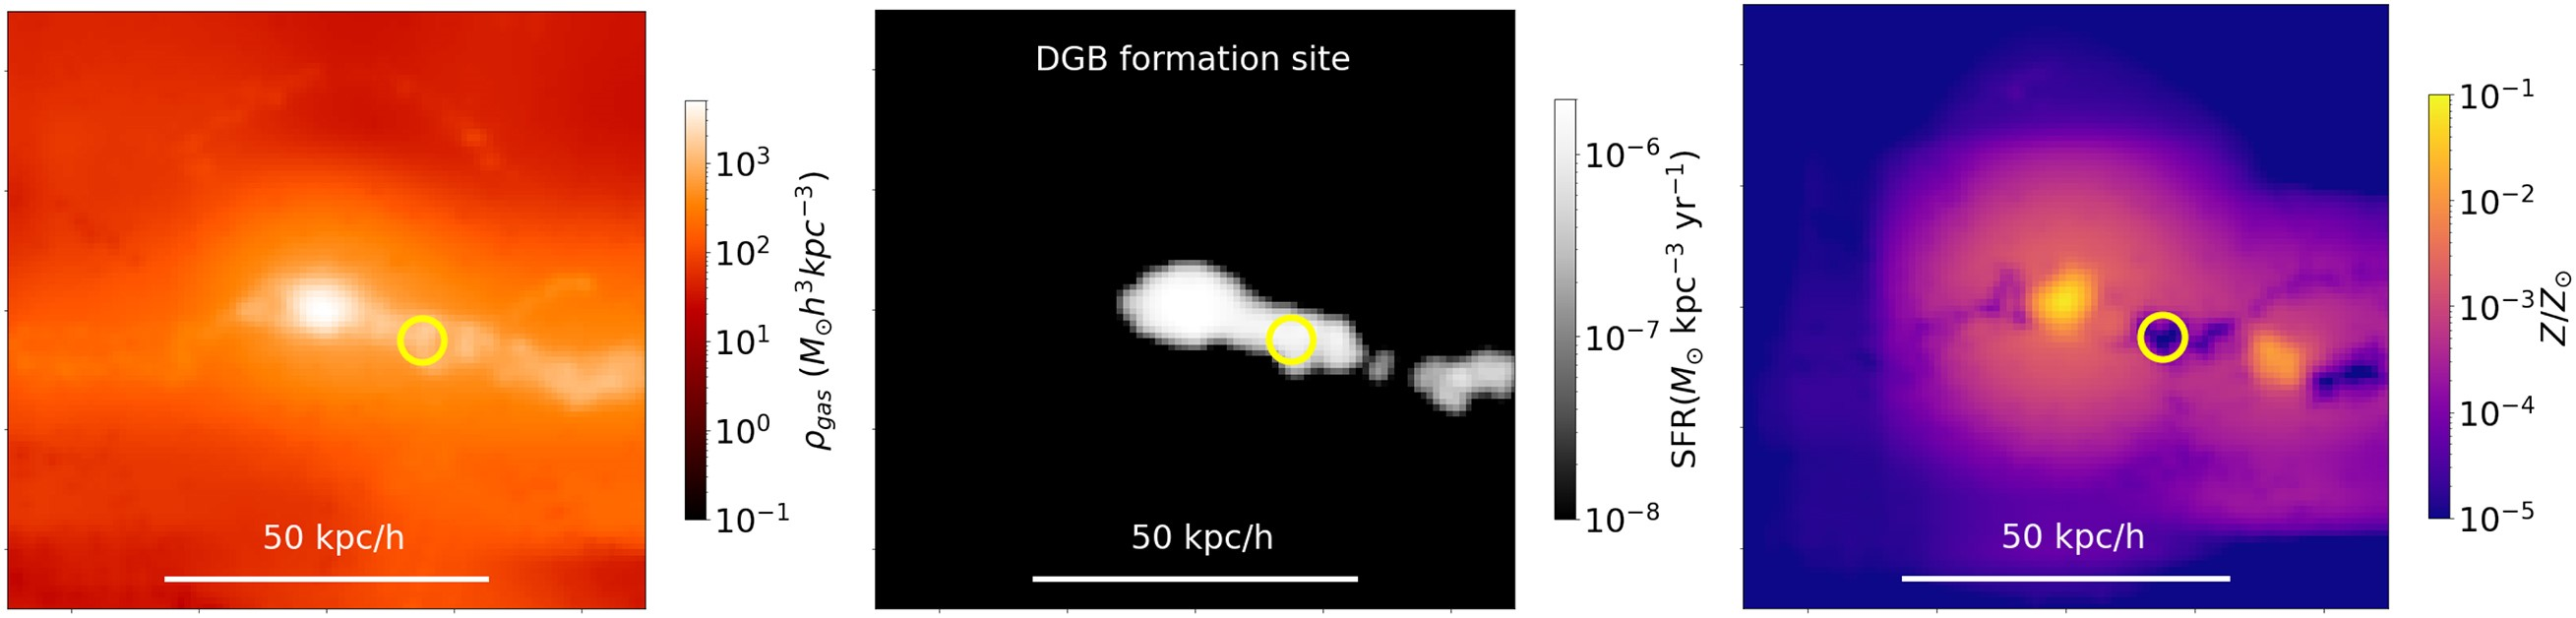
\includegraphics[width=0.9\linewidth]{fig/brahma-seeding.jpeg}
    \caption{An example of the formation site of the gas-based seed model used in BRAHMA. The yellow circle marks the seed formation site comprising of dense and metal poor gas.}
    \label{fig:brahma-seeding-example}
\end{figure}

The BRAHMA simulation suite also consists of runs with seed models that describe heavy seeds \cite{bhowmick2024growthhighredshiftsupermassive}. Heavy seeds are formed from the direct collapse of gas clouds which could happen when fragmentation and star formation is prevented. These 
simulations model $1.2 \times 10^{5}$ \msun{} seeds with additional seeding criteria to describe heavy seeds. Seeds are placed in halos that satisfy the Dense and metal-poor gas mass criterion described above. An additional Lyman-Werner (LW) flux criterion is introduced to require that the dense and metal poor gas mass is also illuminated by a LW flux above a critical value $J_{\rm crit}$. A gas-spin condition is also implemented which is based on the stability analysis of pre-galactic disks and the collapse of unstable disks to form direct collapse black holes \citep{Lodato2006, natarajan2023detectionovermassiveblackhole,Natarajan2012,DeGraf_2019}. Additionally a halo environment criteria is used to ensure that the BHs are forming in rich environments. 


The simulation boxes together probe MBHs within the mass range $\sim 10^3 - 10^7$ \msun{} at $z \geq 7$. Thus, these simulations capture the full mass range observable by LISA and will reduce the uncertainties in MBH merger predictions stemming from mass resolution limitations in previous cosmological simulations. However the above mentioned simulations have very simple prescriptions of the MBH merger dynamics. As the limited mass resolution can create suprious kicks between BHs and nearby particles/cells, most simulations use a respositioning scheme that pins BHs to the gravitational potential minimum. This causes the MBHs to rapidly move to the center of the potential well ater a galaxy merger in unrealistic timescales. To account for the kpc-scale dynamics sub-grid dynamical prescriptions are employed in some simulations \cite{Volonteri_2020,DeGraf_2021}. Even then much of the binary evolution is not accounted for if the two MBHs are assumed to merge when their seperation is within the spatial resolution of the simulations. For most simulations this is of the order of $\sim$ kpc. However, as will be shown in the section below, MBH binaries have a long way to go from $\sim$ kpc till they merge. This calls for the use of sub-grid models that include the MBh dynamics in post-processing these simulations. 


\subsection{Massive black hole binary evolution}
\label{sec:MBHB-evolution}

The dynamics of Massive black holes following a galaxy merger was first studied by the seminal work of \cite{Begelman1980}. At kpc scales,dynamical friction \citep{Chandreshkar1943,antonini_dynamical_2012} is responsible for bringing the MBHs towards the galactic center. The dynamical friction force was on a massive perturber like MBH moving medium composed of collisionless particles was shown by \citet{Chandreshkar1943} to be:

\begin{equation}
    \vec{F}_{\rm DF} \propto - M^2_{BH} \rho \, \mathcal{G} \left(\frac{v}{\sigma} \right) \ln \Lambda \frac{\vec{v}}{v^3}
\end{equation}

where $\rho$  is the background density characterized by an isotropic Maxwellian velocity distribution with velocity dispersion $\sigma$, $v$ is the velocity of the perturber relative to the surrounding background, $\ln \Lambda \sim 10$ is the
Coulomb logarithm and the function $\mathcal{G}(x)$ depends on the underlying velocity distribution.

The MBHB becomes a gravitationally bound system when the mass enclosed by the binary orbit is comparable to the MBH mass, which typically happens around $\lesssim$ 1-10 pc \citep{Begelman1980,Quinlan_1996,Yu_2002}.Once the binary becomes bound, stars with sufficiently low angular momentum  will scatter off the binary and continue to harden it \citep{Sesana_2008,Quinlan_1996,quinlan_dynamical_1997, Merritt_2005}. The region of orbital phase space where stars efficiently scatter with the binary is known as the `loss cone' (LC). Therefore, this phase of hardening is also referred to as `loss-cone' scattering.  The binary becomes ``hard" when its binding energy is comparable to the kinetic energy of the stellar background, and the separation at which this happens is called the hardening radius:

\begin{equation}
    a_{h} = \frac{G \mu}{4 \sigma^2}
\end{equation}

where $\mu$ is the reduced mass of the binary and $\sigma$ is the local velocity dispersion of the surrounding stellar distribution. 

Below this radius, the dynamics are strongly dominated by the self-gravity of the MBHs, resulting in high-velocity ejections of stars and a decrease in stellar density. This, in turn, leads to less frequent stellar encounters. Efficient scattering relies on continuous replenishment of the loss-cone.  If the replenishment due to two-body relaxation is slower than the Hubble time, the binary will stall, causing the so-called ``final parsec problem" \citep{2003MerritandMilosavljevic}. However, Triaxial galactic potentials and galaxy asymmetries can efficiently refill the LC, overcoming this stalling \citep{Yu_2002}. Several other studies have demonstrated that merging galaxies, asymmetric galactic potentials, and galaxy rotation can increase hardening rates \citep{holleybockelmann2006lossconetriaxialgalaxies,berczik_2006,Holley_Bockelmann_2010,Preto_2011,Khan_2011,Holley-Bockelmann2015,Khan_2016}). Even so, stellar loss-cone driven hardening can span several Gyr for some systems \citep{Kelley_2017a}.

At smaller scales ($\lesssim$ 0.1 pc), in gas-rich mergers, binary hardening can happen via interactions with a circumbinary disk (CD) \citep{Dotti_2009,cuadra_massive_2009,nixon_tearing_2013,goicovic_infalling_2017,Siwek2023,Siwek2024}). However, the efficiency of gas-driven hardening in realistic scenarios is uncertain, and it remains unclear whether gas-driven hardening will bring the binary into the mpc regime \citep{lodato_black_2009,moody_hydrodynamic_2019,munoz_circumbinary_2020}. Most mergers detectable in the PTA range originate from low-redshift galaxies, which are typically gas-poor, so gas-driven hardening is less likely to be the primary mechanism for these sources. However, for LISA-detectable mergers, gas interactions are likely more significant as LISA targets MBHBs in the range of $10^4 - 10^7$ \msun \citep{dotti_supermassive_2007}.


Finally, if the above mechanisms are able to bring the MBH binary to below mpc separations, gravitational wave radiation dominates further shrinking of the MBHs until merger. The inspiral driven by GW emission results in secular evolution of the binary oribtal parameters. The semi-major axis and eccentricity evolution in the GW-inspiral is given by equations from \citet{Peters_1963}:

\begin{equation}
 \left(\frac{d a}{dt}\right)_{\rm GW}=-\frac{64G^3}{5c^5} \frac{m_1 m_2 \left	(m_1 +m_2\right)}{a^3} \frac{(1+ 73 e^2/24+ 37e^4/96)}
 {(1-e^2)^{7/2}}.
 \label{dadt_gw}
\end{equation}

\begin{equation}
    \left(\frac{d e}{dt}\right)_{\rm GW}=-\frac{304G^3}{15c^5} \frac{m_1 m_2 \left	(m_1 +m_2\right)}{a^4} \frac{(e+ \frac{121}{304}e^3)}
 {(1-e^2)^{5/2}}
 \label{dedt_gw}
\end{equation}

The hardening mechanisms discussed above leading to a binary MBH coalescence is summarized in figure \ref{fig:path-to-merger}.

\begin{figure}[!htb]
    \centering
    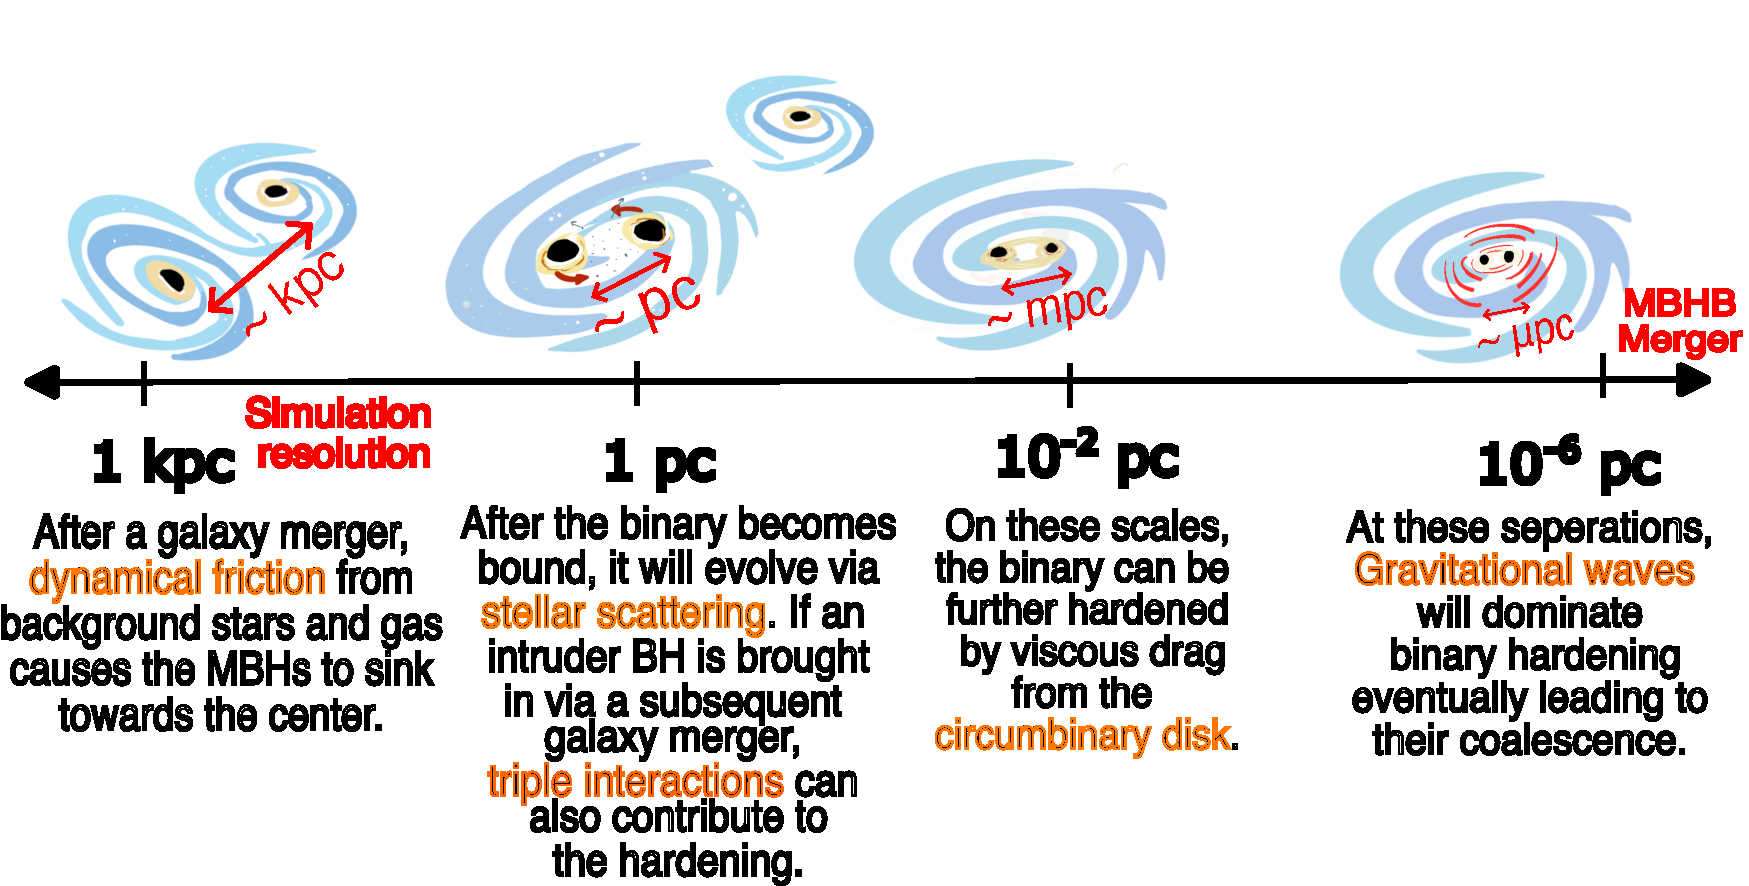
\includegraphics[width=0.9\linewidth]{fig/finesst_1st_fig.pdf}
    \caption{The path to coalescence of an MBH binary. The cosmological simulations have a spatial resolution of $\sim$
kpc, below which several physical processes contribute to the hardening of the binary at various scales and need to be
modeled accurately.}
    \label{fig:path-to-merger}
\end{figure}




\subsection{Triple MBH interactions}
\label{sec: triple-interactions}

Another process that can aid in merging MBHs, particularly if binaries are stalled due to inefficient LC replenishment in gas-poor
environments, involves interactions with a third MBH \citep[e.g.,][]{hoffman_dynamics_2007,ryu_interactions_2017,bonetti_post-newtonian_2018-1}. If the binary inspiral time is long enough to allow a new galaxy merger to bring a third, ``intruder" BH close, then a triple system can form. In hierarchical triple systems, Kozai-Lidov (K-L) oscillations \citep{Kozai1962,Lidov1962,Naoz_2016} can secularly increase the orbital eccentricity of the inner binary, driving it to coalescence. If the intruder reaches the galactic nucleus at distances comparable to the inner binary’s orbital separation, chaotic three-body interactions can trigger a prompt MBH merger. These interactions also frequently result in the ejection of the lightest BH via gravitational slingshot, leaving the more massive pair tightly bound and able to merge on shorter timescales \citep{saslaw_gravitational_1974,hills_encounters_1975,blaes_kozai_2002,iwasawa_evolution_2006,hoffman_dynamics_2007}.


Previous numerical studies of such as \citet{hoffman_dynamics_2007} studied MBH triplets in massive galaxies and showed that three-body interactions enhance the MBHB coalescence rate. They also showed that triple interactions lead to a population of highly-eccentric binaries and also produce a population of `wandering" black holes due to slingshot ejections. Similarly \citet{volonteri_assembly_2003} tracked the formation of triple BHs in halo merger trees and, using a simple prescription of triple interactions, found that slingshot ejections may create a population of wandering black holes.


Although \citet{hoffman_dynamics_2007} used a Newtonian treatment of the dynamics, major improvement were made by \citet{bonetti_post-newtonian_2016,bonetti_post-newtonian_2018-1}, who included relativistic corrections up to 2.5 Post-Newtonian (PN) order in their triple MBH dynamics code and
explored a wide parameter space of triple systems. In a follow-up paper \cite{bonetti_post-newtonian_2018}, they use a semi-analytical model (SAM) of galaxy and massive black hole evolution with triple interaction included by interpolating the numerical simulation results from \citet{bonetti_post-newtonian_2018-1}. 
They found that even if all MBH binaries stall, triple encounters could still produce an observable GWB for PTAs. They also find that the binaries are driven to very large eccentricies, in excess of 0.9 and up to 0.9999 in some cases. Moreover, in a follow-up study, \citet{bonetti_post-newtonian_2019} showed that triple interactions might also significantly contribute to LISA-detectable events. Many of these binaries can also have large eccentricities when entering the LISA
band.

\subsection{Black hole recoil and ejections}
\label{sec:BH-recoil}

BH recoil kicks can also occur following a MBH merger: when merging binaries have unequal masses or spins, they emit asymmetric GW 
radiation, resulting in a GW recoil that displaces the newly merged MBH \citep[e.g.,][]{Bekenstein1973, Campanelli_2007}. Numerical relativity (NR) simulations have shown that GW recoils may reach $\sim$ 5000 \kms \citep{Campanelli_2007,lousto_orbital_2011}. Kicks of even a few hundred \kms\ can eject a MBH from its host galaxy center \citep{Lousto_2012, Gerosa_2014, Ricarte2021} and can potentially impact MBH merger rates. If the MBH is actively accreting at the time of the kick, it will carry along its accretion disk and broad-line region and may appear as an off-center AGN \citep{Loeb_2007,blecha_effects_2008, Volonteri_2008, Komossa_2012}. 

Triple interactions can also produce ejections of the lightest  BH in the triplet via a gravitational slingshot, they may
offset or wandering MBHs, which, in some cases, could manifest as observable offset active galactic nuclei (AGN) \citep{Madau_2004,Loeb_2007, blecha_effects_2008, barrows_spatially_2016, Blecha_2019_Astro2020}. \citet{vanDokkum2023} recently identified a slingshot recoil candidate, but subsequent studies have
favored a bulgeless edge-on galaxy explanation \citep{Sanchez2023,Sanchez2023b,Montes2024}.

A handful of  recoiling AGN candidates have been observed \citep{Komossa2008,Civano2010,Koss2014,Kalfountzou2017,Chiaberge_2017,Hogg_2021,Ward2021,vanDokkum2023,bigmac2024,Uppal_2024}. Conclusive determination of the nature of these candidates has proven difficult, but prominent candidates have been ruled out \citep{Decarli2014,Li2024} and a confirmed recoil has recently been claimed for another candidate \citep{chiaberge2025}. 


The GW recoil kick velocities depend sensitively on the spin vectors of the progenitor MBHs \citep{Gonz_lez_2007,Campanelli_2007,Brugmann_2008,Kesden_2010,Lousto_2012,Berti_2012,Gerosa_2018}. In particular, gas discs can spin up and align the BH spins with the disc prior to the merger, leading to lower recoil velocities \citep{Martin_2007,Bogdanovi__2007,Martin2009,Tremaine2014}. This is mainly due to the Bardeen-Petterson effect that the misalignment between the circumbinary disk and the spin vectors torques the two vectors to align with each other. The accreted matter's angular momentum also changes the spin of the MBH. Conversely, in gas-poor systems the spin misalignment can result in very high recoil velocities. If a recoiling MBH has a velocity greater than the escape speed of the host, then it could lead to an ejection of the MBH. 


Although such ejections may be rare at low redshifts, they could be more common at higher redshifts due to smaller galactic escape speeds and higher merger rates \citep{volonteri_assembly_2003,Blecha2016}. MBH recoil therefore affects MBH growth, MBH-galaxy co-evolution, and the observed scatter in MBH mass-bulge velocity relations \citep{Volonteri_2007,gualandris_ejection_2008,blecha_recoiling_2011}). It also impacts the MBH merger rates detectable by GW observatories like LISA.

% To understand the relative contributions of slingshot kicks and GW recoils in producing wandering and offset BHs, it is important to characterize triple systems and their outcomes. \citet{sayeb_mbh_2023} identified triple MBH populations after applying the binary inspiral model \citet{Kelley_2017a} to the MBH binaries in the Illustris cosmological simulation in post-processing. They identified 
% instances where an intruder MBH overtakes a binary, forming a triple system. Their results show that in their fiducial model,
% 22 \% of the binaries form a triple system, with over $> 70 \%$ being binaries that would not otherwise merge by $z=0$. Additionally, they find that $\sim 6 \%$ of the binaries form ``strong" triples at $\sim$ pc scale separations. 



\subsection{Host galaxy properties}
\label{sec:host-galaxy-properties}
As discussed in the sections above, the MBH binary evolution is strongly tied with the merger environment. For future detection of GWs from MBH binaries, we would like to know which types of host galaxies host them. This will also allow us to look for possible EM counterparts to the GW signal. For example, the circumbinary disk around MBH binaries can produce several EM signatures, many of them producing variations with the binary's orbital period \citep{dorazio2023,dorazio2018,dorazio2015}. When PTAs detect continous GWs from individual MBH binaries, identifying such EM counterparts could provide us key data to understand BH accretion and binary evolution \citep{Kelley_2018}. EM counterparts to LISA GW sources could also be detected, especially at lower redshifts \cite{Bogdanovic_2022}. Therefore, characterization of the host galaxies of MBH binaries is very important. 

Previous works have used cosmological simulation, like the Illustris simulation to look for characteristics of host environments of MBH mergers \citep{DeGraf_2021}. They found that morphological evidence of a recent galaxy merger may persist for $\sim 500$ Myrs in PTA-like sources ($M > 10^8$ \msun{}). However, the time between the galaxy merger and PTA detection might be such that such identification of morphological features are unlikely. They also found that their sample of host galaxies of MBH mergers at $z<8$ are not a biased population of galaxies. The low-mass mergers are found to have enhanced specific star formation rate (sSFR), but the high mass mergers specific SFR seems to be unaffected. This work, however assumed a fixed time delay between the galaxy merger and the BH merger.

More recently \citet{Cella_2024} used the Illustris simulation along with a post-processing semi-analytic model of MBHB evolution to determine the properties of the host galaxies of likely PTA hosts. They use a GW detection probability to the MBHB sources to weigh the host galaxy characteristics. They find that the detectable sources have host galaxy properties that are distinct from the overall galaxy population. Figure \ref{fig:PTA-host-properties} shows the properties of the host galaxies weighted with detectability of the consistent MBHB by PTA from this work. The peak stellar mass in the host galaxies weighted by GW detection probability shifts from $\sim 10^{10}$ \msun{} to $\sim 10^{12}$ \msun{}, by two orders of magnitude. The peak of the stellar metallicity for host galaxies with detectable GWs sources is $\sim 2 Z_{\odot}$, comapred to the peak of $\sim 0.6 Z_{\odot}$ in the overall distribution of binary host galaxies. This is most likely because the galaxies experiencing major mergers and hosting an MBHB massive enough to be detectable by PTAs tend to be older. The plot also shows sSFR for the binary hosts with GW detectable binaries drop by an order of magnitude compared to all host galaxies. \citet{Cella_2024} also shows that galaxies hosting MBHBs detectable by PTAs tend to be redder and brighter, implying they are likely to be quenched ellipticals with diminshed star formation rates. 


\begin{figure}
    \centering
    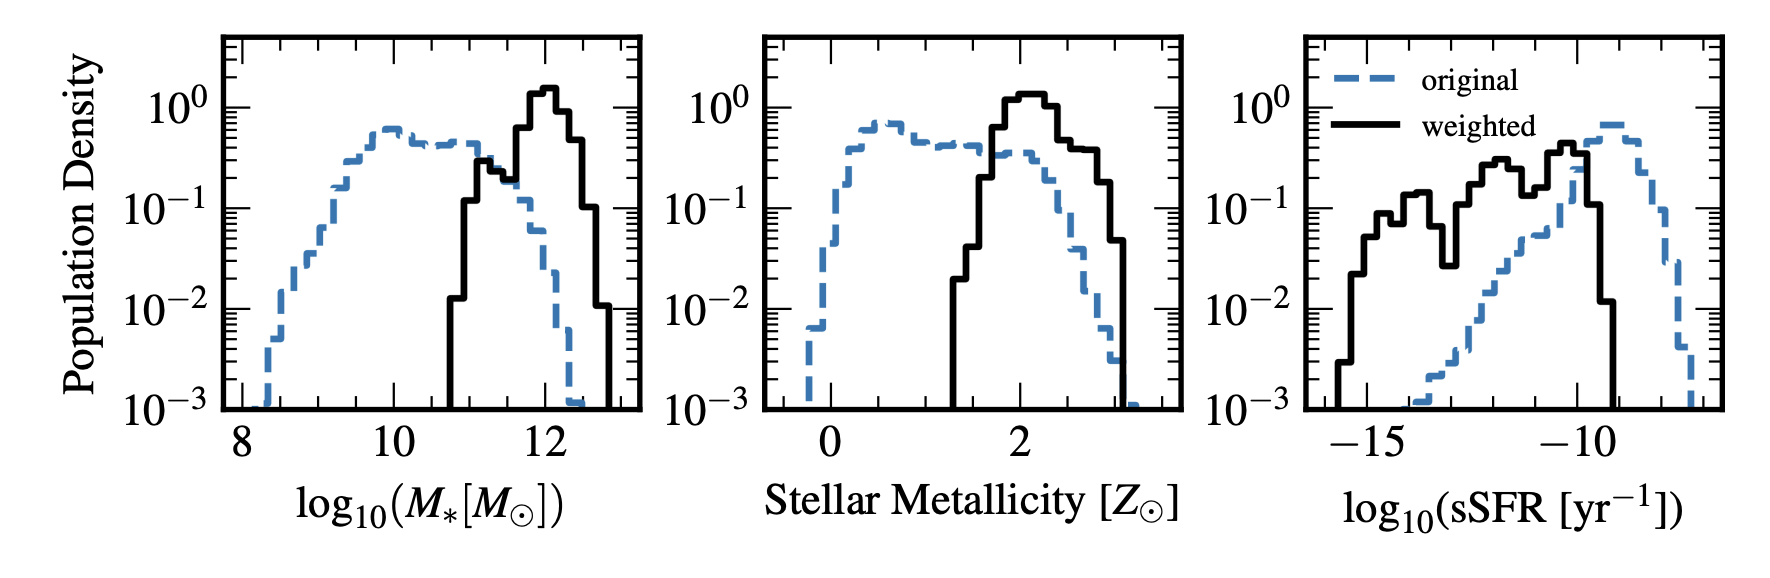
\includegraphics[width=0.9\linewidth]{fig/host_property_PTA.png}
    \caption{Distribution of the stellar mass, stellar metallicity and specific star formation rate for the unweighted host galaxy properties and the weighted host galaxies with the GW-detectability of their binary MBHs from \citet{Cella_2024}.}
    \label{fig:PTA-host-properties}
\end{figure}


It should be noted that a lot of these characteristics of host galaxies with GW-detectable binaries are a result of scaling relations. A more general study of galaxies post-merger with a MBHB needs to be conducted with high resolution cosmological simulations. There is also a lot of certainty in the host galaxy properties at higher redshifts, like the association of AGN fueling and galaxy mergers \citep{Cisternas2011,Villforth2017,Bhowmick2020}. At higher redshifts, the BHs and the host galaxies retain signatures of their origins, making it particularly interesting to characterize the properties merging environments in the early universe. High-resolution simulations at these redshifts \citep{bhowmick2024introducingbrahmasimulationsuite} would provide valuable insights into the host galaxy propoerites in the early universe. 

\section{Modeling MBH dynamics in cosmological simulations}
\label{sec:MBH-dynamics-project}

Since cosmological simulations like Illustris cannot probe dynamics below the scale of the gravitational softening length defined for each particle or cell, the dynamics of the binary inspiral need to be modeled beyond the simulation resolution. To achieve this, we apply the post-processing models of \citet{Kelley_2017a,sayeb_massive_2021}. These models use inward extrapolation of host galaxy density profiles and compute the hardening rates of binary inspiral due to dynamical friction, stellar scattering, circumbinary gas-disk driven hardening, and GW emission. \citet{sayeb_mbh_2023} explore potential triple MBH systems by investigating MBHs that experience more than one merge and identifying the subset that are most likely to experience strong triple interactions. For the first project, we take this sub-population of likely strong triples and model their outcomes by incorporating the triple interaction subgrid model from the \citet{bonetti_post-newtonian_2016,bonetti_post-newtonian_2018} numerical simulations of MBH triplets to model their outcomes.

\subsection{Methods}

\subsubsection{MBH binary inspiral model}
\label{sec: insp-hardening-model}
The time when the MBH merges in Illustris is called the binary \emph{formation time}, after which we apply the post-processing inspiral models of  \citet{Kelley_2017a}. The MBH population considered here is the same as the one in \citet{sayeb_massive_2021} and \cite{sayeb_mbh_2023}. Illustris uses a repositioning scheme which pins MBHs to the potential minimum of their host halos. The effects of this are most problematic for small 
satellite halos that are spuriously re-seeded with MBHs after losing their initial MBH during an interaction with a larger halo. As this predominantly affects MBHs close to the seed mass, we follow previous work and exclude
MBHs below $10^6$ \msun{}.  The inspiral model also requires a binary to have a reasonably well resolved host galaxy in the snapshots before and after the merger for calculating the environmental effects for calculating hardening rates. This adds additional constraints of a minimum of 80 gas cells, 80 star particles, and 300 DM particles. All of these constraints reduce the subset of 23708 MBH mergers in Illustris to 9234 systems \citep{Kelley_2017a,sayeb_massive_2021,sayeb_mbh_2023}. The binary inspiral model evolves these binaries through four different hardening mechanisms \citep{Begelman1980}: dynamical friction (DF), loss cone scattering (LC), hardening due to circumbinary disk (CD), and hardening via gravitational wave radiation (GW). The hardening time scales for the different mechanisms is shown in figure \ref{fig:hardening-time-scales}.


\begin{figure}[!htb]
    \centering
    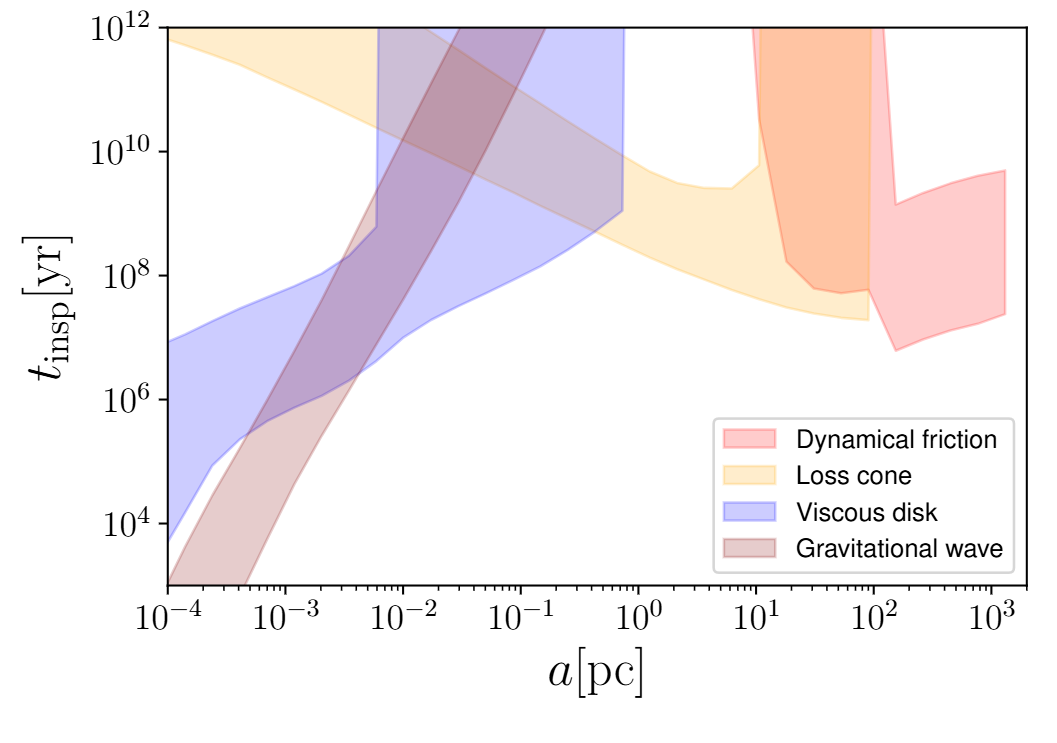
\includegraphics[width=0.7\linewidth]{fig/hardening_time_scales.png}
    \caption{Hardening time scales versus binary separation for different mechanism calculated as $a (da/dt)^{-1}$. DF starts to dominate binary hardening at a few kpc up to a few pc where LC dominates. Stellar scattering dominates until a few hundredth of a pc after which CD and GW dominates at smaller separations. }
    \label{fig:hardening-time-scales}
\end{figure}

Our fiducial model assumes a full loss cone and allows for the eccentricity to vary in the LC phase. The LC hardening rate $da/dt$ and the eccentricity evolution $de/dt$ is based on the scattering experiments by \citet{Sesana_2006} and are as follows:


\begin{align}
    \left( \frac{da}{dt} \right)_{\rm LC} &= - \frac{G \rho}{\sigma} a^2 H\\
    \left( \frac{de}{dt} \right)_{\rm LC} &= \frac{G \rho}{\sigma} a H K
    \label{dadt_lc}
\end{align}

where $a$ is the binary separation, $e$ is the orbital eccentricity. $\rho$ and $\sigma$ correspond to the stellar density and the stellar velocity dispersion profiles of the host in Illustris. $H$ and $K$ are dimensionless constants set by numerical scattering experiments and here we use the values from \citet{Sesana_2006}. The initial eccentricity of all binaries is set to be $e_{0} = 0.6$ at the beginning of the DF phase in our fiducial model. The eccentricity is evolved during the LC and GW-dominated phase. The GW hardening rate and the eccentricity evolution follows Equations \ref{dadt_gw} and \ref{dedt_gw}. Note that, we do not include eccentricity evolution in the CD phase. 

 \subsubsection{Triple interaction outcomes}
\label{sec:triple-outcomes}
\begin{figure}[!htb]
    \centering
    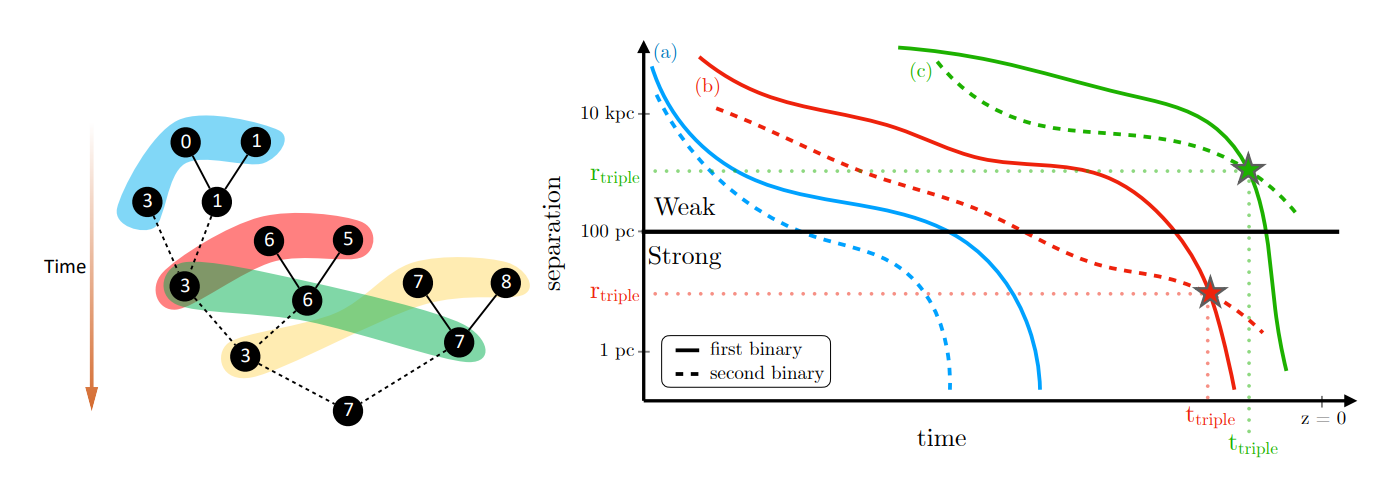
\includegraphics[width=0.9\linewidth]{fig/triple-MBH-identification.png}
    \caption{(Left): An example of a Merger tree where each circle represents a unique ID in Ilustris and the highlighted areas indicate potential triple systems. To look for triple systems, we search for repeated IDs in the merger tree. (Right
    ): The binary separation vs time for the inner binary (Solid lines) and the outer binaries (dashed lines). If the curves cross at a time before $z=0$, then the system becomes a successful triple. The blue curve shows a failed triple system, the red curves show a strong triple system, formed at small separations ($a <100$ pc) and the green curves represent a weak triple formed at large separations ($a>100$ pc). Figure from \cite{sayeb_mbh_2023}.}
    \label{fig:trip-identify}
\end{figure}

Although the binary inspiral model evolves each binary in isolation, we can identify binary systems sharing a common MBH in the merger tree. If the binary inspiral times of the two binaries overlap, they are considered co-existing binaries and may represent a potential triple system. 

Out of the sample of co-existing binaries, we denote the binary with the earliest formation time as the `first' or inner binary and the `second' or 'outer' binary is the one with the later formation time. A triple system is defined as one for which the separation of the outer binary becomes smaller than that of the inner binary at a given point in time, which we identify as the triple formation time
$t_{\rm triple}$, and the corresponding separation at which the outer binary overtakes the inner binary is called the triple formation radius $a_{\text{triple}}$ (see Figure \ref{fig:trip-identify}). Triples with $a_{\text{triple}} > 100$ pc are classified as `weak triples' and triples with $a_{\text{triple}} > 100$ pc are `strong triples'. The cutoff between strong and weak triples is set at 100 pc and is validated through K-means clustering applied to all the triples.
Because the strong triples are more likely to undergo three-body interactions, we choose to focus only on strong triples for our exploration of the outcomes of triple interactions. 


Once the triples have been identified from the Illustris binaries, the next step is to find the masses of the BHs in the binary $m_1$, $m_2$ and the intruder BH mass $m_3$. To identify these BHs, we first calculate the expected mass of the merger product. This is done by summing the masses of the original binary components, $m_1$ and $m_2$, and the total mass accreted by the binary between its formation and the time of triple formation. Let $\Delta m$ represent this accreted mass, calculated using the black hole accretion rates from Illustris. The expected mass of the merger product is then $m_{\rm prod} = m_1 + m_2 + \Delta m$. Among the two BHs in the second binary, we identify the one with mass closest to $m_{\rm prod}$ as the merger product. The other BH is then classified as the intruder, with mass denoted by $m_3$.

We also account for the mass growth for the individual BHs in the first binary. To calculate the mass accreted by each BHs in the first binary, we assume that the accretion onto each BH is proportional to their masses. The new primary and secondary masses become:
\begin{eqnarray}
    \label{eq: m1m2 accreted mass}
    m_{1} \rightarrow m_{1} +  \Delta m/(1+q)\\
    m_{2} \rightarrow  m_{2} +  \Delta m  \, q / (1+q)
\end{eqnarray}

After finding the mass growth of each BH of the inner binary, we consider the maximum of the two masses to be the primary and the minimum to be secondary (i.e $m_1 = \max (m_1,m_2)$ and vice-versa). Once we obtain the set of strong triples and their masses ($m_1,m_2,m_3$), we incorporate triple dynamics with the help of results from the triple MBH simulations from \citet{bonetti_post-newtonian_2018-1}. 



The outcomes of triple MBH interactions in \citet{bonetti_post-newtonian_2018-1} are sampled for different values of primary mass $m_1$ sampled in the range [ $10^5$ \msun{}, $10^{10}$ \msun{}] and inner mass ratio $q_{\rm in} \in [0.03,1]$ and outer mass ratio $q_{\rm out} \in [0.03,1]$ . They also perform a set of simulations for the case where the intruder is more massive than the MBHB, i.e $q_{\rm out} > 1$ systems. The simulation is performed for systems with different inner and outer orbit eccentricities and relative inclinations. For each simulation grid point, three merger fractions for the merger of $m_1-m_2$, $m_1-m_3$, and $m_2-m_3$ represented by $a,b,c$ are recorded. Similar to \citet{bonetti_post-newtonian_2018}, we perform grid interpolation between our set of strong triples represented by $(m_1, q_{in}, q_{out})$ and the surveyed points from the simulation to obtain the merger fractions $a,b,c$  for the strong triples. To decide the outcome of the strong triple interaction, a random number P is chosen between 0 and 1, and one of the two choices is considered:

\begin{itemize}
    \item A \emph{prompt merger} of one of the pairs in the triple system triggered by the triple interaction and a the lightest BH kicked out when $P \leq a+b+c$. 

    \item For $P > a+b+c$, the lightest MBH is kicked due to gravitational slingshot from the triple interactions. The remaining binary will evolve further after the kick.
\end{itemize}

We perform 100 realizations of the outcomes for the strong triple population. To further evaluate the merger time, we need to evolve the binaries after the triple interaction. For \emph{prompt mergers}, \citet{bonetti_post-newtonian_2018-1} shows that the time spent by strong triples before merger can be fitted with a log-normal distribution, with a mean $\mu = 8.4$ and standard deviation $\sigma = 0.4$ in $\log(T/yr)$. We add a merger time sampled from this distribution to $t_{\rm triple}$ to get the prompt merger time.

\begin{figure}
    \centering
    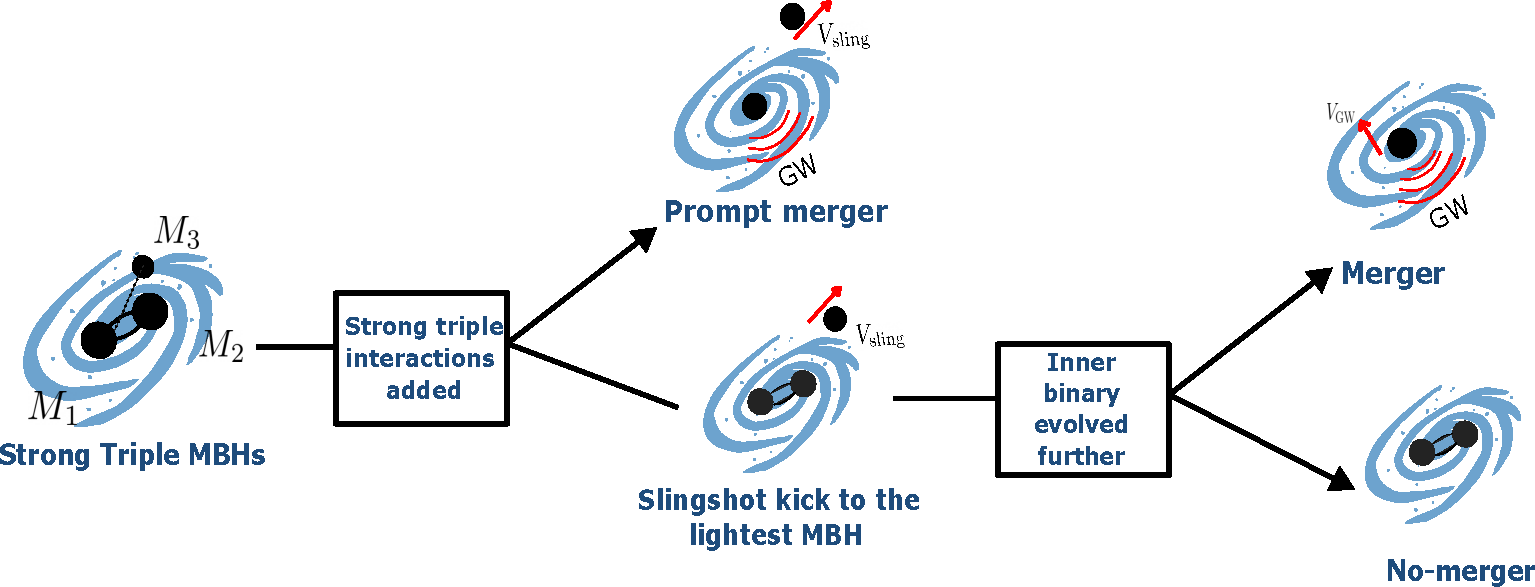
\includegraphics[width=0.9\linewidth]{fig/strong_triple_interactions_outcomes_for_paper.pdf}
    \caption{The outcomes of binary and triple interactions in our population. Strong triple interactions are only added for the strong triple subpopulation ($a<100$ pc).}
    \label{fig:Triple-outcomes}
\end{figure}
In cases where the lightest BH is kicked from the triple system and there is no prompt merger, the leftover binary may coalesce within a Hubble time, though this is not always the case. \citet{bonetti_post-newtonian_2018-1} saw that the remaining binaries that merge via GW emission constitute  20\% %$1/5$ th 
of the total merger fraction in triple systems. In cases of a light intruder, after it gets scattered via gravitational slingshot, the remaining binary is hardened. The new binary seperation of the inner binary is then calculated following \citet{volonteri_assembly_2003}. In the case of a heavier intruder that causes an exchange interaction, it would replace the secondary MBH in the inner binary. We therefore evolve the outer binary in this case with the new calculated binary separation. If $t_{\rm merger}<t_{\rm H}$, we call such cases \emph{merger after kick}. The systems that do not merge within Hubble time are stalled and hence added to the \emph{no-merger} case. These outcomes are shown in Figure \ref{fig:Triple-outcomes}. Note that because weak triples (formed at separations $>100$ pc) are unlikely to undergo three-body interactions, we do not include these systems in the calculations of the triple interaction outcomes. However, any mergers between BHs in these systems that occur via normal binary inspiral are counted in the total merger population.
Note that the binary can have a higher orbital eccentricity after the triple interaction. Although eccentricity is included in the binary evolution model, we are not currently evolving them after the triple interaction. In \citet{bonetti_post-newtonian_2018}, eccentricity was assigned to the triples from the eccentricity distribution from the triple MBH recorded at an arbitrary point close to their merger. In future work, we will employ a more accurate eccentricity and inspiral evolution coupled with strong triple interactions.

We also consider a ``stalled" model, where all potential triple systems from Illustris are assumed to stall at the time of binary formation. We then apply the triple interaction subgrid model to these systems, averaging over 100 realizations of the outcomes and look for prompt mergers. This model, similar to the \emph{Model-stalled} in \citet{bonetti_post-newtonian_2018}, allows us to assess the role of triple interactions in facilitating mergers when binaries would otherwise remain stalled.

\subsubsection{Calculation of GW recoil}
\label{sec:GW-recoil-calculation}
The merger of two MBHs with unequal masses or spins will result in a GW recoil to the merger remnant. The GW recoil velocity depends on the spins and the mass ratio of the merging BHs.  The mass ratio is calculated for the merging BHs and the BH spins are drawn from physically motivated distributions. If the inspiral is driven by torques from a circumbinary gas disk, the BH spins tend to align with the orbital angular momentum preferentially \citep{Bogdanovi__2007, Dotti2010,Miller_2013}. Whereas, in gas poor systems where the inspiral is primarily driven by stellar interactions, the resulting spin orientations may tend to be random \citep{Merritt_2012}. As we are unsure of the efficiency of these processes in various merger environments, we pick three spin distributions for different spin orientations and magnitudes for the MBH population. 

\begin{figure}[htb!]
    \centering
    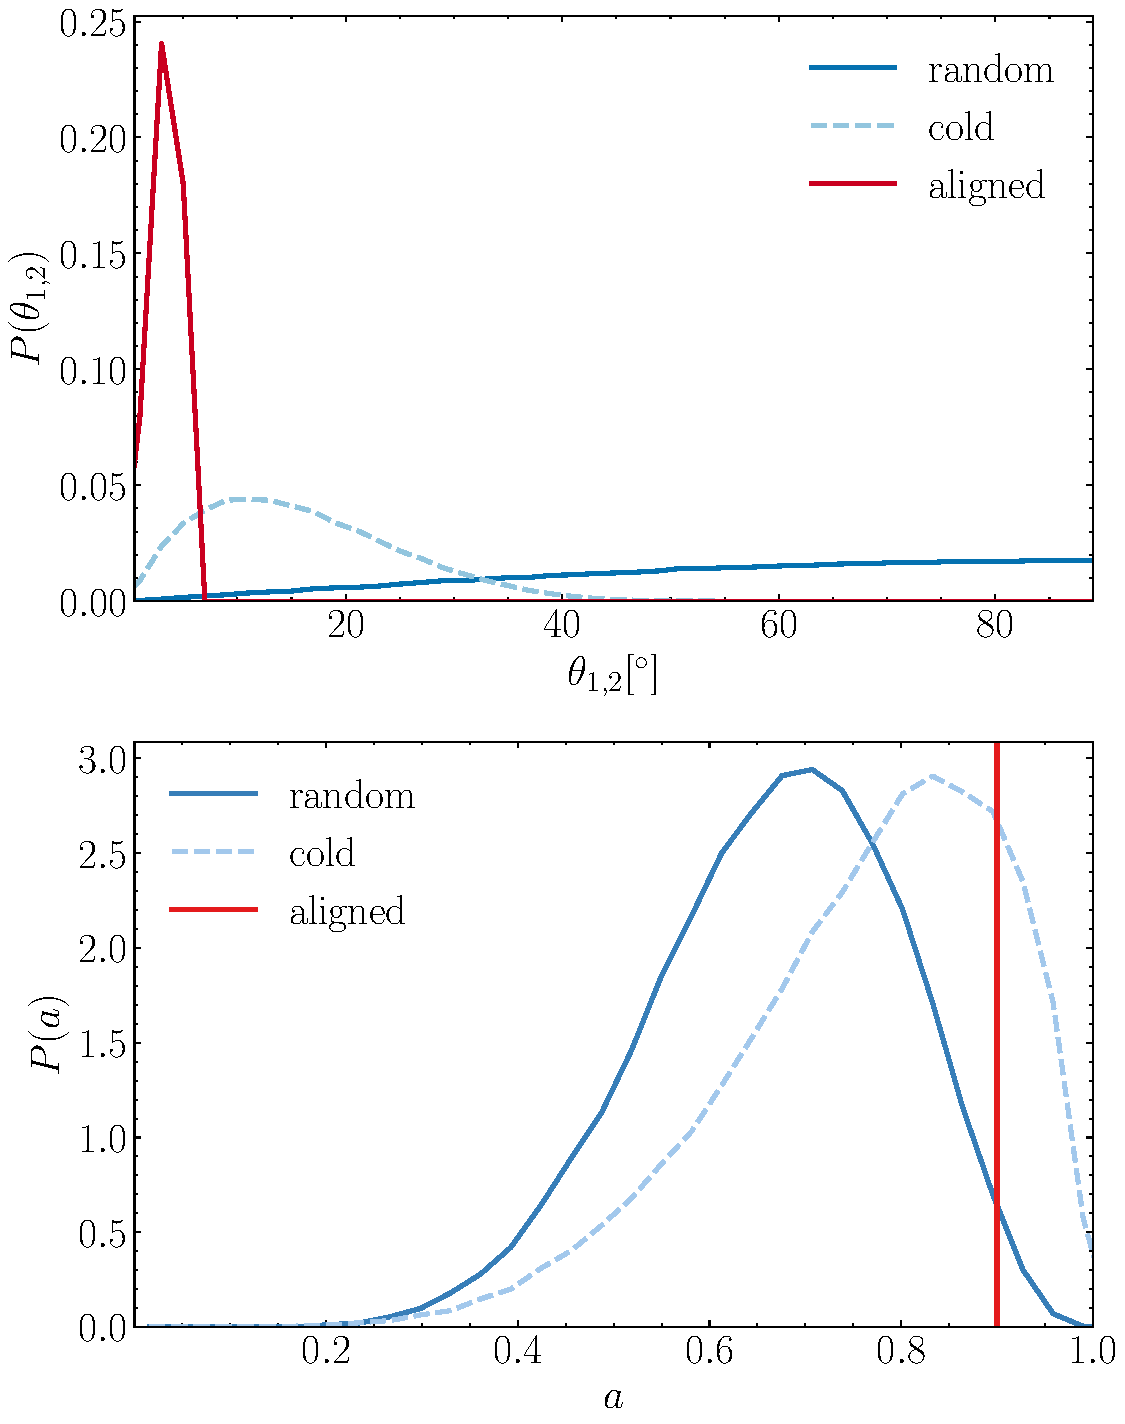
\includegraphics[scale=0.45]{fig/spin-models-magnitude-and-angle.pdf}
    \caption{Normalized distributions of the three spin models considered in this work: \texttt{random} (solid dark blue), \texttt{cold} (dotted light blue), and \texttt{deg5} (solid red). \textit{Top panel:} misalignment angle distribution of the spins. \textit{Bottom panel:} spin magnitude distribution of the models.}
    \label{fig:spin-dist}
\end{figure}


The three spin models considered here are from \cite{Blecha2016}. The first spin model produces a random spin distribution as a result of successive dry mergers. The spin magnitude is represented by a beta distribution that peaks at $a \sim 0.7$ \citep{Lousto_2012} and has a large tail towards low spins (Figure \ref{fig:spin-dist}). The spin misalignment angle $\theta$ (relative to the orbital angular momentum) is drawn randomly in the interval $(0^{\circ},180^{\circ})$. This model is called \texttt{random-dry} but for the sake of simplicity we will refer to it as \texttt{random}. It is represented by the dark-blue curve in Figure \ref{fig:spin-dist}. At the other extreme, we can assume the spins are always highly aligned before the merger. To represent this choice, we consider the misalignment angle chosen over the interval $(0^{\circ},5^{\circ})$ and a high spin magnitude ($a = 0.9$). This spin model is called the \texttt{aligned} and is represented by the red lines in Figure \ref{fig:spin-dist}.

In the third spin model, we take the cold gas fraction of the progenitor halos into consideration. As the BH spins may be aligned due to the presence of a circumbinary gas disk, we assume that gas-rich galaxy mergers likely trigger the formation of a massive circumbinary disk. We define a ``gas-rich" galaxy as one with cold (star-forming) gas fraction $f_{\text{gas,sf}}> 10 \%$. The gas fraction is defined as $f_{\text{gas,sf}} = M_{\text{gas,sf}}/(M_{*} + M_{\text{gas,sf}})$ where the $M_{\text{gas,sf}}$ and $M_{*}$ are the gas mass and stellar mass within the stellar half-mass radius of the progenitors. The majority of galaxies in our population (more than $85 \%$) are gas-rich. The gas-rich mergers would then have BH spins drawn from a \texttt{cold} spin evolution model described in \cite{Dotti2010} and \cite{Lousto_2012}. This model represents the case of the nearly aligned spin ($\lesssim10^{\circ}$) and is represented by the dotted blue lines in figure \ref{fig:spin-dist}. For gas-poor mergers with $f_{\text{gas,sf}} <  10 \%$, the spins are drawn from the \texttt{random} described above. We call this the \texttt{hybrid} spin model and it is represented by the blue dotted lines in Figure \ref{fig:spin-dist}.

Once the progenitor BH spins are drawn from the distribution for a given spin model, the recoil kick velocity is calculated using a fitting formula from \cite{Lousto_2012}, which is based on numerical relativity simulations:

\begin{equation}
{\mathbf v_{\rm recoil}} = v_{\rm m}  {\mathbf {\hat e}_{\perp,1}}+ v_{\perp} ({\rm cos} \,\xi \, {\mathbf {\hat e}_{\perp,1}} + {\rm sin} \,\xi \, {\mathbf {\hat e}_{\perp,2}}) + v_{\parallel} {\mathbf {\hat e}_{\parallel}},
\label{eqn:kick}
\end{equation}
\begin{equation}
v_{\rm m} = A \eta^2 \sqrt{1 - 4\eta} \,(1 + B \eta), 
\end{equation}
\begin{equation}
v_{\perp} = {H \eta^2 \over (1 + q )} (a_{2\parallel} - q a_{1\parallel}),
\end{equation}
\begin{eqnarray}
v_{\parallel} = {16 \eta^2 \over (1+ q)} \left [ V_{1,1} + V_{\rm A} \tilde S_{\parallel} + V_{\rm B} \tilde S_{\parallel}^2 + V_{\rm C}\tilde S_{\parallel}^3 \right ] \times \\ \nonumber 
|\, {\mathbf a_{2\perp}} - q {\mathbf a_{1\perp}} | \, {\rm cos}(\phi_{\Delta} - \phi_1),
\end{eqnarray}

where $\eta \equiv q/(1+q)^2$ is the symmetric mass ratio, $\perp$ and $\parallel$ refer to vector components perpendicular and parallel to the orbital angular momentum, respectively, and ${\mathbf {\hat e}_{\perp,1}}$ and ${\mathbf {\hat e}_{\perp,2}}$ are orthogonal unit vectors in the orbital plane. The vector ${\mathbf {\tilde S}} \equiv 2({\mathbf a_2} + q^2 {\mathbf a_1})/(1+q)^2$, and $\phi_{\Delta}$ is the angle between the in-plane component ${\mathbf \Delta_{\perp}}$ of the vector ${\mathbf \Delta} \equiv M^2({\mathbf a_2} - q {\mathbf a_1})/(1+q)$ and the infall direction at merger. The phase angle $\phi_1$ depends on the initial conditions of the binary and is assumed to be random. The best-fit values of $A = 1.2\times 10^4$ \kms, $B = -0.93$, $H = 6.9\times10^3$ \kms, and $\xi = 145^{\circ}$ are taken from \cite{Gonz_lez_2007} and \cite{Lousto2008}, and the coefficients $V_{1,1} = 3677.76$, $V_{\rm A} = 2481.21$, $V_{\rm B} = 1792.45$, and $V_{\rm C} = 1506.52$ (all in km s$^{-1}$) are defined in \cite{Lousto_2012}.


\subsubsection{Slingshot kick calculation}
\label{sec: slingshot-kick}

If the intruder BH $m_3$ is smaller than both the BHs ($m_1,m_2$) in the inner binary, then the triple encounter will likely lead to the scatter of the intruder BH. The intruder is kicked due to gravitational slingshot and the binary recoils by momentum conservation. The binary orbit shrinks as a result of the encounter. The binding energy for such encounters increases by the amount $\langle\Delta E/ E_B\rangle = 0.4 (m_3/(m_1 + m_2))$ \citep{Hills1980}, where $E_B$ is the binding energy of the binary. In cases where the intruder MBH is more massive than the binary components ($m_3 > m_2$ or $m_3 > m_1$), there will likely be an exchange event with the lightest BH ejected and the remaining two forming a binary. In both the cases there is an increase in the binding energy of the BH pair. For outer mass ratios $q_{out} \leq 2$, most of the increase in binding energy is due to shrinking of the orbit whereas for $q_{out} > 2$, the increase is mainly due to the change in mass due to the exchange of a low mass member by a more massive BH \citep{volonteri_assembly_2003}. 

The binding energy $E_B$ is calculated at the triple formation time when the strong interactions take over. The separation at the triple formation time is denoted by 
$a_{\rm triple}$. However, this value would be an overestimate for the actual separation where ejection happens. The binary could instead evolve to the hardening radius $a_h$ \citep{quinlan_dynamical_1997,Begelman1980}. To account for this, we take the minimum of the two separations for the separation to get the separation during gravitational slingshot recoil, $a_{0} = min(a_h, a_{t})$.

The change in binding energy is calculated by the same scheme used by \cite{volonteri_assembly_2003}. The scheme is summarized as follows:

\begin{itemize}
    \item If $m_3<m_2$, $m_3$ is scattered of leaving with $\langle\Delta E/ E_B\rangle = 0.4 \, q_{out}$  and a new semi-major axis $a_1 = a_0/(1+0.4 q_{out})$
    \item If $m_3 > m_2$ and $q_{out} < 2$, it will result with an exchange event with $\langle\Delta E/ E_B\rangle = 0.4 \, q_{out}$ 
    and a new semi-major axis $a_1 = a_0 (m_3/m_2)/(1+0.4 q_{out})$
    \item If $q_{out} > 2$, an exchange happens with $\langle\Delta E/ E_B\rangle = 0.9$ and a new semi-major axis $a_1 = 0.53 a_0 (m_3/m_2)$.
\end{itemize}

The kinetic energy of the ejected BH through gravitational slingshot will then be:

\begin{equation}
    K_{ej} = \frac{\Delta E}{1 + (m_{\text{ej}}/m_{\text{bin}})}
    \label{eq: K_ej}
\end{equation}

where $m_{\text{ej}}$ is the mass of the lightest BH among the three and $m_{\text{bin}} = m_1 + m_2$ is the mass of the final binary. Hence, during scattering $m_{\text{ej}} = m_{3}$ and $m_{\text{bin}} = m_1 + m_2$ and during exchange  $m_{\text{ej}} = m_{2}$ and $m_{\text{bin}} = m_3 + m_1$. The gravitational slingshot kick velocity is calculated from Equation \ref{eq: K_ej} and the orbital separation after the strong triple interaction is updated. The binary after the kick is evolved further if it didn't merge via through prompt-merger (as described in Section \ref{sec: triple outcomes}). If a binary remains after the triple interaction, this updated separation is used as the starting point to model its continued inspiral.

\subsubsection{MBH ejections}
\label{sec: BH ejections}

The kicked BH needs to have a velocity larger than the escape velocity $v_{esc}$ for it to be ejected. To count the number of possible ejections from both GW kicks and slingshot kicks, the escape velocity of the host galaxy is computed. For the DM component, we assume a simple \cite{Hernquist1990} potential $\Phi(r) = - G M_{DM} / (r + r_H)$, where $M_{DM}$ is the sum of the DM masses of the progenitor subhalos of the merging MBHs and $r_H$ is the scale radius. $r_H$ is related to the half mass radius by $r_{\rm half} \approx 2.414 \, r_{H}$  .The stellar component is modeled using a softened isothermal density profile, $\rho_{*} = \sigma_{*}^{2}/(2 \pi G (r^2 + r^2_{\text{soft}}))$, with velocity dispersion $\sigma^2_{*} = G M_{*}/R_{\text{bulge}}$ and $r_{\text{soft}} = G M_{BH}/\sigma^{2}_{*}$. We take the stellar bulge truncated at an outer radius $R_{\text{bulge}}$ to be a simple average of the progenitor stellar half-mass radii. The potential of merging galaxies is however dynamic and major mergers in particular can drastically change the structure of the progenitors. \cite{blecha_recoiling_2011} have shown that the escape velocity $v_{esc} $ is volatile during a merger and in some cases $v_{esc}$ increases during the merger.

A BH is counted as ejected if the recoil kick from either GW recoil or slingshot kick is larger than the central escape speed of the host galaxy. An ejected BH's ID is checked for repetition in the merger tree and any subsequent merger that this BH undergoes is discarded. 



\subsection{Results}


\subsubsection{Properties of the merger population}
\label{sec:merger-properties}

\begin{figure*}[!htb] 
    \centering
    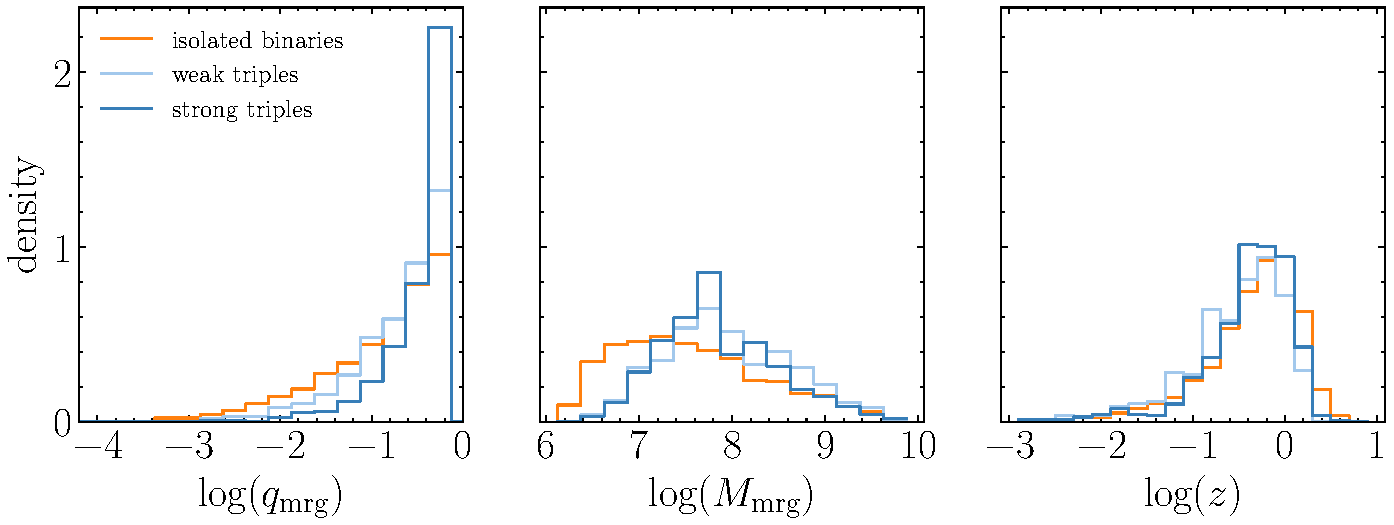
\includegraphics[scale=0.7]{fig/mrg_properties_hist.pdf}
    \caption{Distributions of the merging BH mass ratio ($q_{\text{mrg}}$), total mass ($M_{\text{mrg}}$), and redshift ($z$) of the merging MBHs in the isolated binaries, weak triples, and strong triples subpopulations.}
    \label{fig:merger-properties-hist}
\end{figure*}


The fiducial model has 9234 binary systems, out of which 22 \% (2029) form triple MBH systems. The remainder, which we call isolated binaries, are systems that evolve entirely in isolation. Of the 2029 triples in the population,
520 (26 \%) are strong triples and 1509 (74 \%) are weak triples (\SB{}). The mergers in isolated binaries are found by tracking their evolution via the inspiral model described in Section \ref{sec: insp-hardening-model}. Mergers induced by strong triple interactions are identified for 100 realizations of each strong triple system, as described in Section \ref{sec:triple-outcomes}. The mergers in weak triples are determined by the inspiral timescale of the inner binary. We do not account for strong triple interactions in the weak triple subpopulation.


In Figure \ref{fig:merger-properties-hist}, we show the normalized mass ratio ($q_{\text{mrg}}$), the total mass ($M_{\text{mrg}}$), and the redshift ($\log z$) of the merging MBHs in the three distinct subpopulations. The median mass ratio for mergers resulting from strong triples, $q_{\text{mrg}} = 0.61$, is significantly higher than the mass ratio of isolated binary mergers ($q_{\text{mrg}} = 0.25$). About 64 \% of strong triple mergers are major mergers with $q_{\text{mrg}} > 0.1$. Mergers resulting from triple interactions are also more massive than isolated mergers; the median mass of merging MBHs in isolated binaries is $3.89 \times 10^7 M_{\odot}$ versus $7.83 \times 10^7 M_{\odot}$ for strong triples.
This is largely because massive galaxies (hosting more massive MBHs) experience more mergers and are thus more likely to host triple MBH systems.
For the weak triples, the median mass ratio is 0.4, and the median  $M_{\text{mrg}} = 9.72 \times 10^7 M_{\odot}$. This reflects the finding in \SB{} that among triples, weak triples are found in massive systems and have lower mass ratios compared to strong triples. Such systems often occur when two satellite galaxies (each carrying a low-mass MBH) fall into the same massive central galaxy.


21 \% of strong triple interactions result in a \emph{prompt merger} of two BHs and a slingshot kick to the other BH, which is often the lightest in the system.  In other cases, a slingshot kick to the lightest BH may not be accompanied by a prompt merger of the remaining BHs, but this remaining binary could still subsequently merge, often on a shorter timescale as a result of the triple interaction. Such \emph{merger after kick} events occurs in 48 \% of strong triples. Thus, a total 69 \% of strong triple systems result in a merger event by $z=0$. Before including triple dynamics, we find that only 40\% (210) of strong triple systems have an inner binary resulting in a merger via inspiral evolution. Thus, strong triple dynamics raise the merger fraction of this binary sub-population from 40\% to 69 \%.

The merger fraction seen in the \emph{merger after kick} scenario is much higher compared to the \cite{bonetti_post-newtonian_2018} simulations. This is because the post-ejection mergers in their simulations are calculated by considering only GW-induced inspiral. We evolve the binary using our hardening model initialized from an updated, closer binary separation after the triple interaction, as described in Section \ref{sec: triple outcomes}. This leads to many cases where the leftover binary coalesces after the slingshot kick. 


We also do not consider the eccentricity evolution of the inner binaries. Triple interactions can make the binary extremely eccentric and in \cite{bonetti_post-newtonian_2019}, they assign eccentricities to the triples from the distribution found through the simulations. The kicked MBH could also fall back into the galactic potential and merge with the binary merger remnant in some cases \citep{hoffman_dynamics_2007}. This could potentially provide some additional mergers in strong triples.

\begin{figure*}[!htb] 
    \centering
    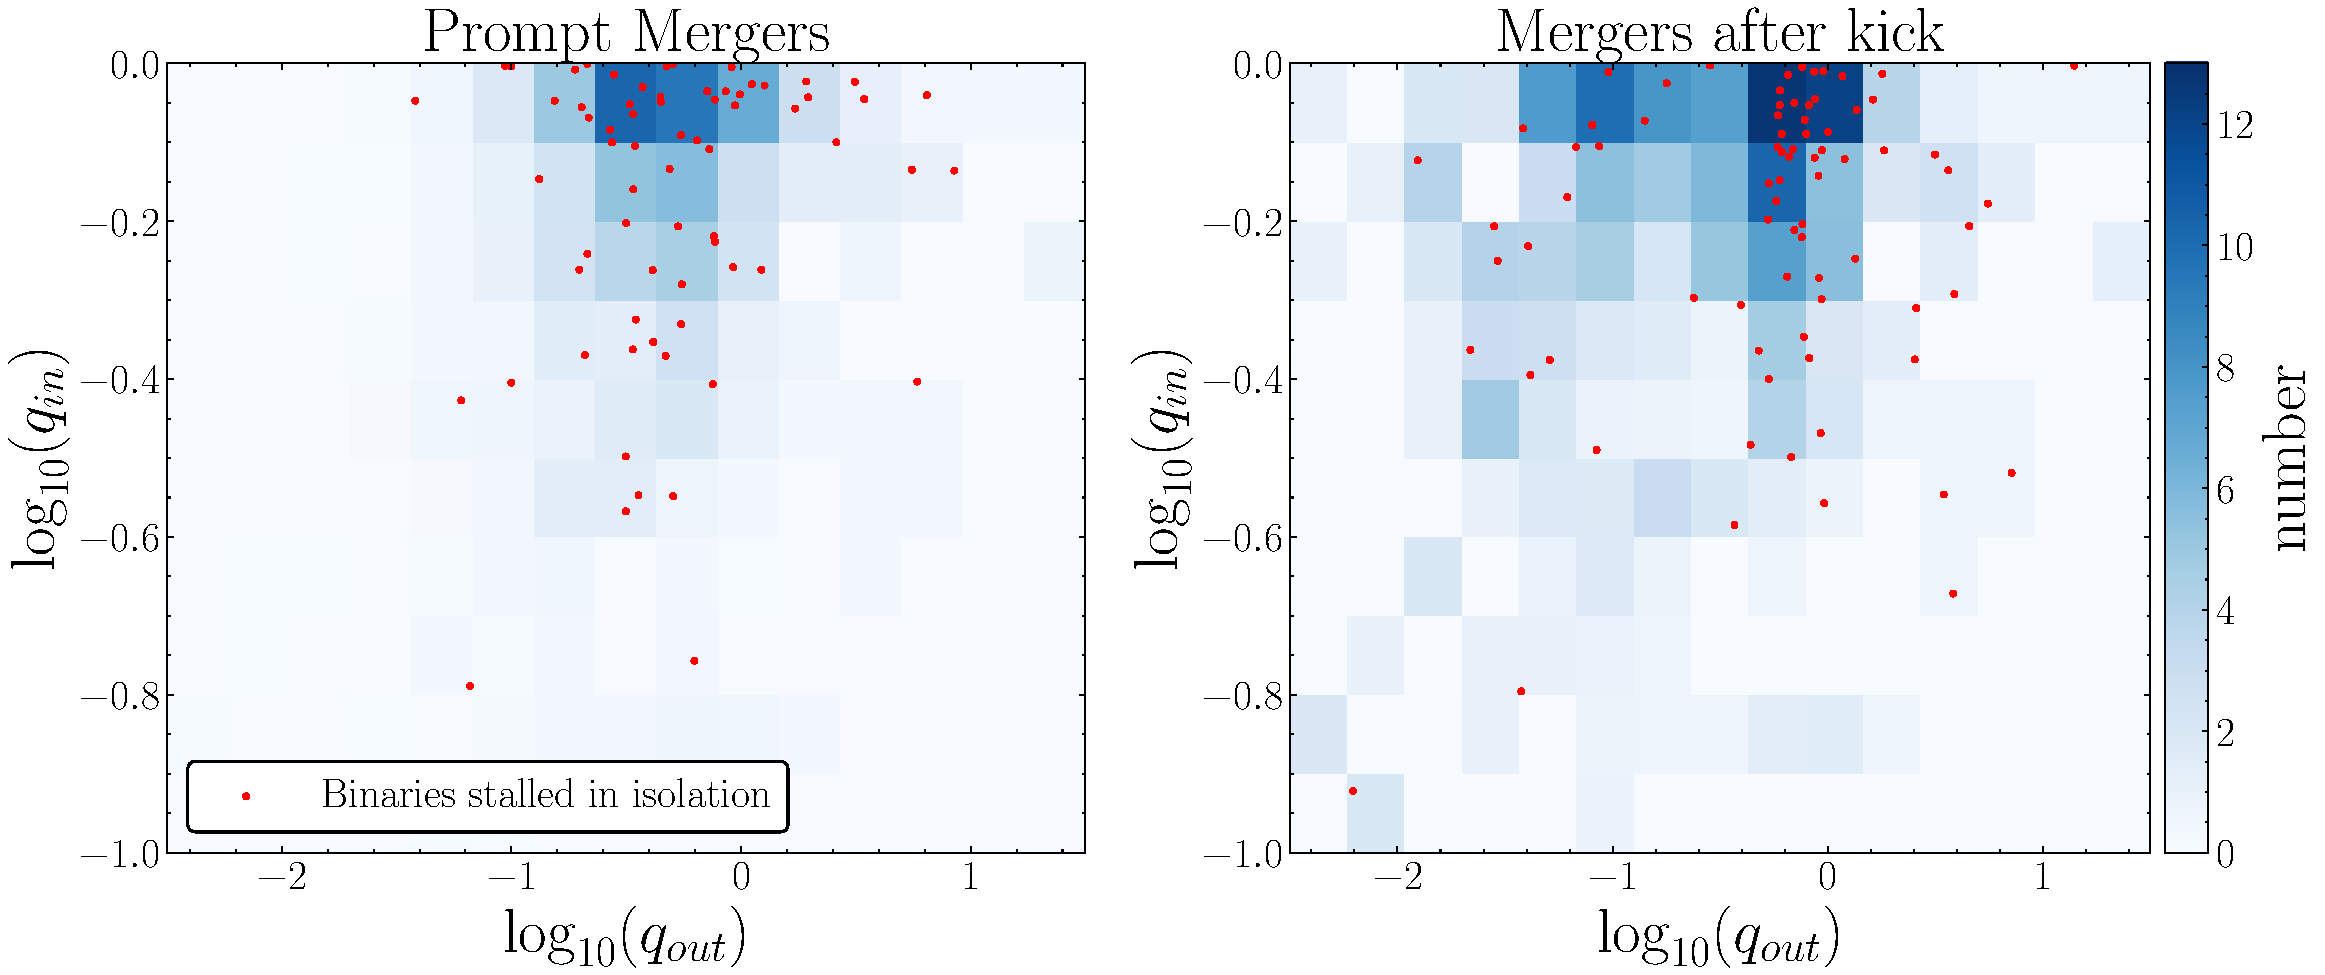
\includegraphics[scale=0.4]{fig/2d-hist-qin-qout-for-mergers.pdf}
    \caption{A 2D histogram in the $\log q_{\text{in}} - \log q_{\text{out}}$ plane for i) prompt mergers and ii) merger after a slingshot kick from triple interactions. The red dots correspond to system where the inner binary would not have merged in isolation.}
    \label{fig:2d-hist-qin-qout}
\end{figure*}


Figure \ref{fig:2d-hist-qin-qout} illustrates the number of mergers in the $\log q_{\rm in}$ - $\log q_{\rm out}$ plane for the \emph{prompt merger} and \emph{merger after kick} cases in strong triples. The prompt mergers peak around equal-mass triplets ($\log q_{\rm in} \sim 0$ and $\log q_{\rm out} \sim -0.3) $, similar to what is observed in \citet{bonetti_post-newtonian_2018}. This is because comparable-mass triples will have the strongest interactions, as opposed to systems with less massive intruders that may be ejected with minimal perturbation to the inner binary. We also show the distribution of triple systems that would not have merged in isolation in the same plot (red dots). Note that $q_{\rm out} > 1$ always corresponds to an exchange event where the intruder replaces the secondary in the inner binary.


\subsubsection{Merger rates}
\label{sec:merger-rates}

\begin{figure*}[!htb] 
    \centering
    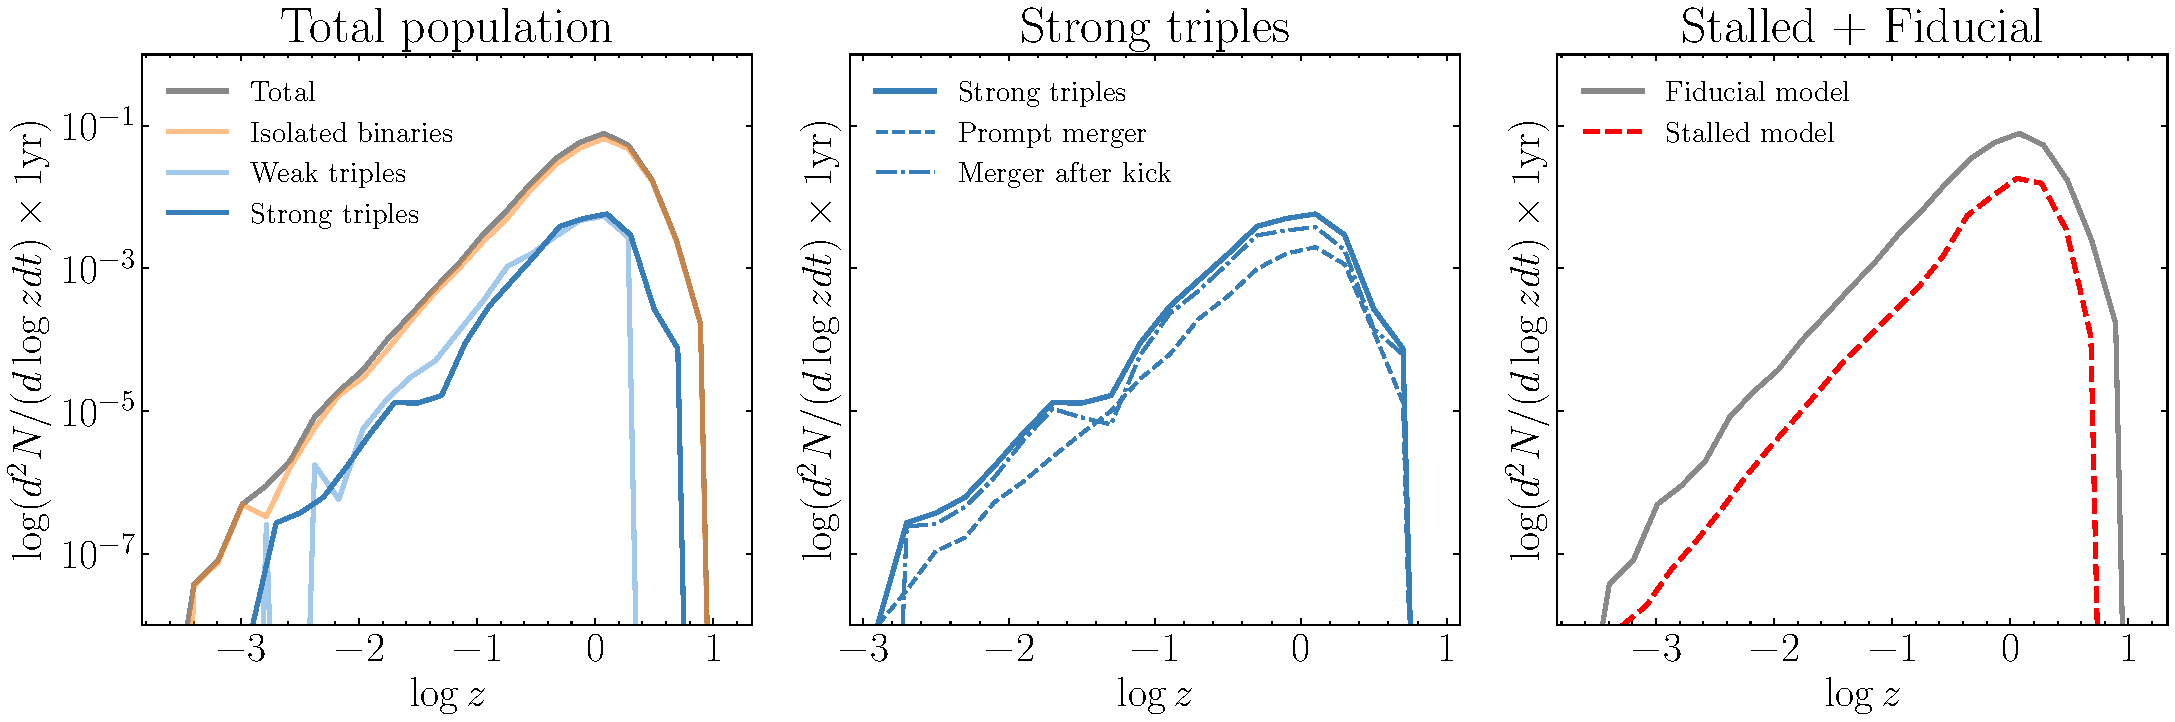
\includegraphics[scale=0.45]{fig/Merger_rate_w_stalled_N_100.pdf}
    \caption{Merger rates of the total population of MBHBs in i) the fiducial model, ii) strong triple subpopulation and iii) comparison of stalled and fiducial model. The grey solid line is the fiducial model's total merger rate, and the red dotted line is the merger rate in the stalled model. The orange solid line is for isolated binaries and the light blue line is for binary merger in weak triples. The solid dark blue line is the total MBHB mergers in strong triples averaged over all realizations of their outcomes. In ii) we also show the merger rates for the two outcomes of strong triple interaction: \emph{prompt merger} and \emph{merger after kick}.}     
    \label{fig:merger-rates}
\end{figure*}


We now focus on the merger rate of the MBHs in the total population and subpopulation and asses the impact of the triple interactions on the overall merger rate. We calculate the differential merger rate as follows: 

\begin{equation}
\frac{d^2N}{d \log{z} \, dt_{\text{obs}}} = \frac{1}{1+z} \frac{dN}{d \log{z}} \left( \frac{1}{V_c}\frac{d V_c}{dz}\right) \frac{d z}{dt}    
\label{eq: merger rate}
\end{equation}

where $d^2N/(d \log{z} \, dt_{\text{obs}})$ is the number of merging binaries that would be observed between $\log{z}$ and $\log{z} + d \log{z}$, over a time-interval $dt_{\text{obs}}$ in the observer frame. $\frac{dN}{d \log{z}} \left( \frac{1}{V_c}\frac{d V_c}{dz}\right)$ is the co-moving number density of mergers in the simulation per unit $\log{z}$ interval. The $\frac{1}{1+z}$ factor converts the time interval from the rest frame of the merger to the observer's frame. For the sake of simplicity, we will refer to this as `merger rates'.

Figure \ref{fig:merger-rates} shows the merger rates for the fiducial and stalled models along with the sub-population of strong triples, weak triples, and isolated binaries. The grey line is the fiducial model's total merger rate, and the red dotted line corresponds to the merger rate in the stalled model. In the fiducial model, the isolated binaries dominate the mergers as expected as they are $78 \%$ of the population. The total merger rate of isolated binaries is $0.13$ yr$^{-1}$ and the cumulative merger rate at $z=0$ overall cosmic time is $0.37$ yr$^{-1}$. The solid dark blue line corresponds to the merger rate of strong triples. The redshifts for the strong triple mergers are found from the time of their merger which is calculated as described in Section \ref{sec:triple-outcomes}. The cumulative merger rate (at $z=0$) in strong triples is  $ 0.018$ yr$^{-1}$. The solid light blue line represents the binary mergers that occur in weak triple systems. They give a cumulative merger rate of $ 0.017$  yr$^{-1}$. The mergers from strong triples thus are $5 \%$ of all the mergers in the fiducial model.

It is interesting to note that the total strong triple merger rate is comparable to the binary merger rate in weak triple systems, even though the number of strong triple systems ($520$) is lower than the weak triple systems ($1509$) and thus shows the efficiency of strong triple interactions in producing mergers. The total merger rate with strong triple interaction is $0.15$ yr$^{-1}$ and the cumulative merger rate at $z=0$ over all cosmic time is $0.40$ yr$^{-1}$. The merger rates are in agreement with \cite{Blecha2016} and the \emph{Model-delayed} in \cite{bonetti_post-newtonian_2019}. 

It should be also noted that some of the isolated binaries were part of coexisting binary systems that didn't form a triple (referred to as failed triple in \SB{}). In the majority of these systems, the inner binary merges before the outer binary overtakes. It could be possible that some of these systems would have come close to forming a triple system. Of these, \SB{} looks for systems with a small binary separation ratio ($1 < (a_2/a_1)_{\text{min}} \leq 10$) and also a close inner binary at the point of closest approach ($a_1 < 100$ pc) and such systems are only 1\% of the total binary population. These near misses therefore at best could give a small enhancement to the strong triple merger rates. 

In the stalled model, all 9234 binaries are assumed to stall unless they merge via triple interactions. $42$ \% of all MBHs are involved in more than one merger over Hubble time. We consider strong triple interactions in all such systems assuming that the intruder BH comes close enough to form a triple system. This model is similar to the \emph{Model-stalled} in \cite{bonetti_post-newtonian_2019} where the MBHs are stalled at the hardening radius and only allowed to merge through three-body interactions. We find that a total of 812 systems (9 \% of the total population) undergo a prompt merger triggered via triple interactions. The total merger rate of triple systems in the stalled model is $0.032$ yr$^{-1}$. Note that, there could be some merger after the triple interaction via inspiral but as we are not evolving the binaries in isolation for this model, we ignore them here. We compare the merger rates of the stalled model (solid grey line) to the fiducial model (dotted red line) in Fig \ref{fig:merger-rates}. Compared to the total merger rate of the fiducial model, this merger rate is only suppressed by a factor of 4.6. \cite{bonetti_post-newtonian_2019} also estimate similar merger rates for their \emph{Model-stalled} and \emph{Model-delayed} models. They also calculate the GWB background in both of their models at the relevant frequency range for PTAs and see that the GWB in the stalled model is only suppressed by a factor of 2-3. Therefore, we verify that even if all the binaries stall, triple interactions prevent the merger rate from dropping too low to produce an observable GWB.

\begin{figure}[!htb] 
    \centering
    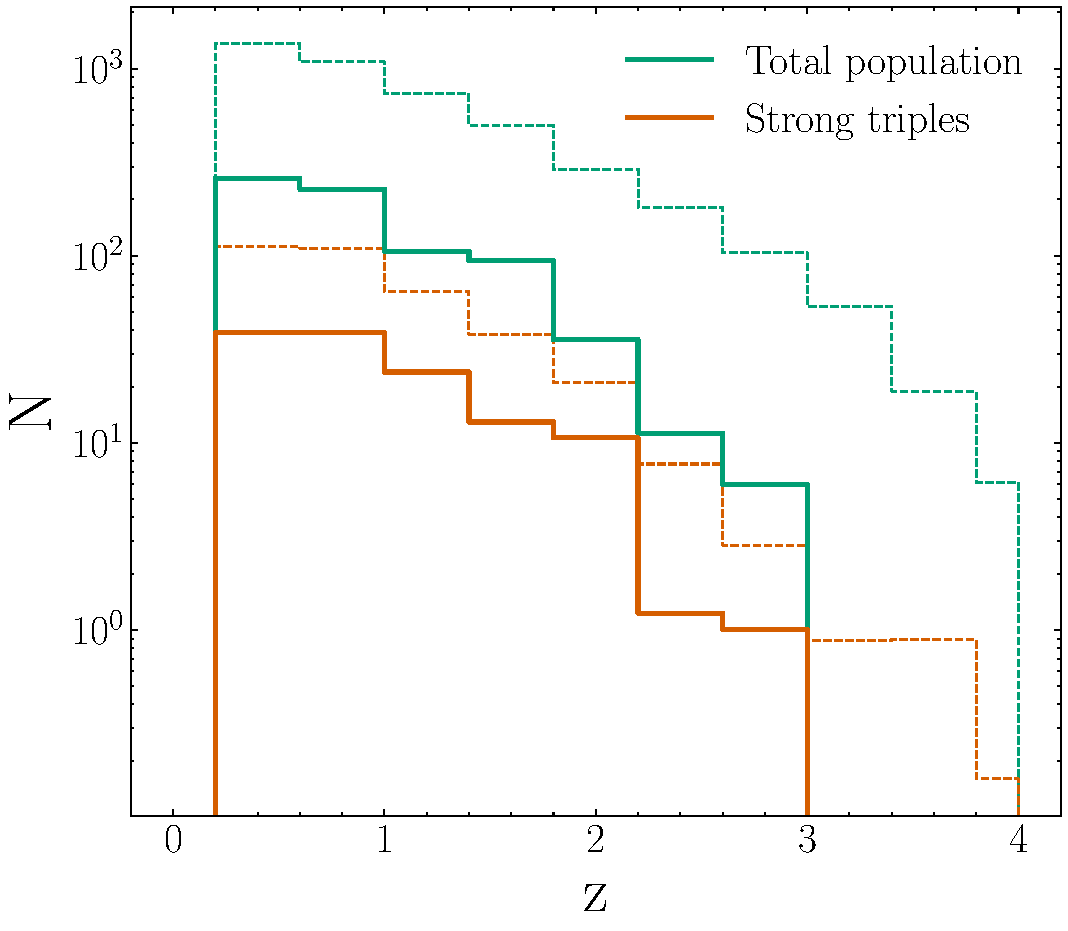
\includegraphics[scale=0.45]{fig/strong_triple_massive_major_mergers_N.pdf}
    \caption{Number of massive major mergers in strong triples (solid orange) and massive major mergers in the total population (solid green) compared to the number of total mergers (dotted orange) and mergers in strong triples (dotted green). Strong triple mergers contribute to 19 \% of the massive major merger population. Here, massive major mergers stand for $M_{\text{mrg}} > 10^8 M_{\odot}$ and $q_{\text{mrg}} > 0.1$.}
    \label{fig:massive-major-mergers}
\end{figure}

Although we are not computing the GWB associated with strong triples in this work, we investigate the presence of massive major mergers in the population. Massive, major MBH mergers will be the loudest GW events observable with PTAs \citep{Barausse_2020}). Here, we look at $M_{\text{mrg}} > 10^8 M_{\odot}$ and $q_{\text{mrg}} > 0.1$ as the massive major subpopulation. 

We see that $53.6 \%$ of mergers in strong triple are major mergers. Also, strong triples contribute to $17 \%$ of the massive major mergers in the total population. This is in contrast to the $5 \%$ contribution of the strong triples observed in the total population. In Figure \ref{fig:massive-major-mergers} the number of massive, major mergers for strong triples and the total population are shown in solid lines, while the dotted line indicates all mergers for both populations. The relative contribution of massive, major mergers by strong triples (solid-orange) is seen to be higher than their contribution in total mergers. However, we do not observe a strong redshift dependence in the fractional contribution of strong triple mergers in massive major mergers. 

This implies that triples have a significant contribution to the MBH merger events observed in PTAs. This result also reflects the distribution of the $M_{\text{mrg}}$ and $q_{\text{mrg}}$ of the triples compared to the isolated binaries in Figure \ref{fig:merger-properties-hist}. Triple interactions are therefore important for massive major and this is because massive galaxies have higher chances of experiencing a second merger in their lifetimes. Hence why such systems form triples as the MBHB timescales are typically longer than the time between the galaxy mergers. This was also observed in \cite{bonetti_post-newtonian_2018} where a large fraction of the mergers in the very high mass range are due to the triple channel. 



\subsubsection{Recoil kicks}
\label{sec:recoil-kicks-result}

We now turn our attention to the recoil events in our population, happening due to gravitational wave recoil and slingshot kicks. As described in Section \ref{sec:GW-recoil-calculation}, we have considered three different spin configurations for our BHs: \texttt{random}, \texttt{hybrid}, and \texttt{aligned} spins. We calculate the GW recoil kick assuming spins drawn from each of these distributions, averaging over 10 realizations per case. For triple systems, the slingshot kick velocity is calculated through the method outlined in Section \ref{sec: triple kick calculation}. We also assign GW recoil kicks for the merged BH in the triple systems by the same procedure as isolated binaries. 

Figure \ref{fig:kick-distributions-for-GW-recoil-and-slingshot} shows the distribution of kick velocities obtained for all spin models - \texttt{random}, \texttt{aligned}, \texttt{hybrid}, and slingshot kicks. GW recoil kicks are shown as averaged distributions over 10 spin realizations, with a 1-$\sigma$ spread indicated. The maximum kick velocities produced by GW recoil are 3190.33 \kms for \texttt{random} spins, 2750.22 \kms for \texttt{hybrid} spins, and 610.68 \kms for \texttt{aligned} spins, averaged over the realizations. Slingshot kicks yield a maximum kick magnitude of 8149.61 \kms. Both GW recoil kicks from \texttt{random} spins and slingshot kicks dominate the high-velocity range, with 14\% and 12\% of their kicks exceeding 1000 \kms, respectively. However, only $1$ \% of kicks in the hybrid spin model are above 1000 \kms and $9$ \% of them are above 500 \kms. The aligned spin model only produces $0.5$ \% of kicks above 500 \kms. The median GW recoil velocities are 282 \kms, 132 \kms, and 106 \kms for \texttt{random}, \texttt{hybrid}, and \texttt{aligned} spins, respectively, while slingshot kicks yield a median velocity of 301 \kms.

Although slingshot kicks can reach extreme velocities, their overall occurrence is limited, as strong triples comprise only 6\% of the population. Around the 600 \kms threshold, the number of GW recoil kicks from the \texttt{aligned} spin model becomes comparable to slingshot kicks. At velocities exceeding 3100 \kms, slingshot kicks surpass GW recoil kicks from \texttt{random} spins. Given that the maximum GW recoil velocity for \texttt{random} spins is around 3190 \kms, any kick above this threshold is likely due to gravitational slingshot effects from triple MBH interactions.


\begin{figure*}[!htb]
    \centering
    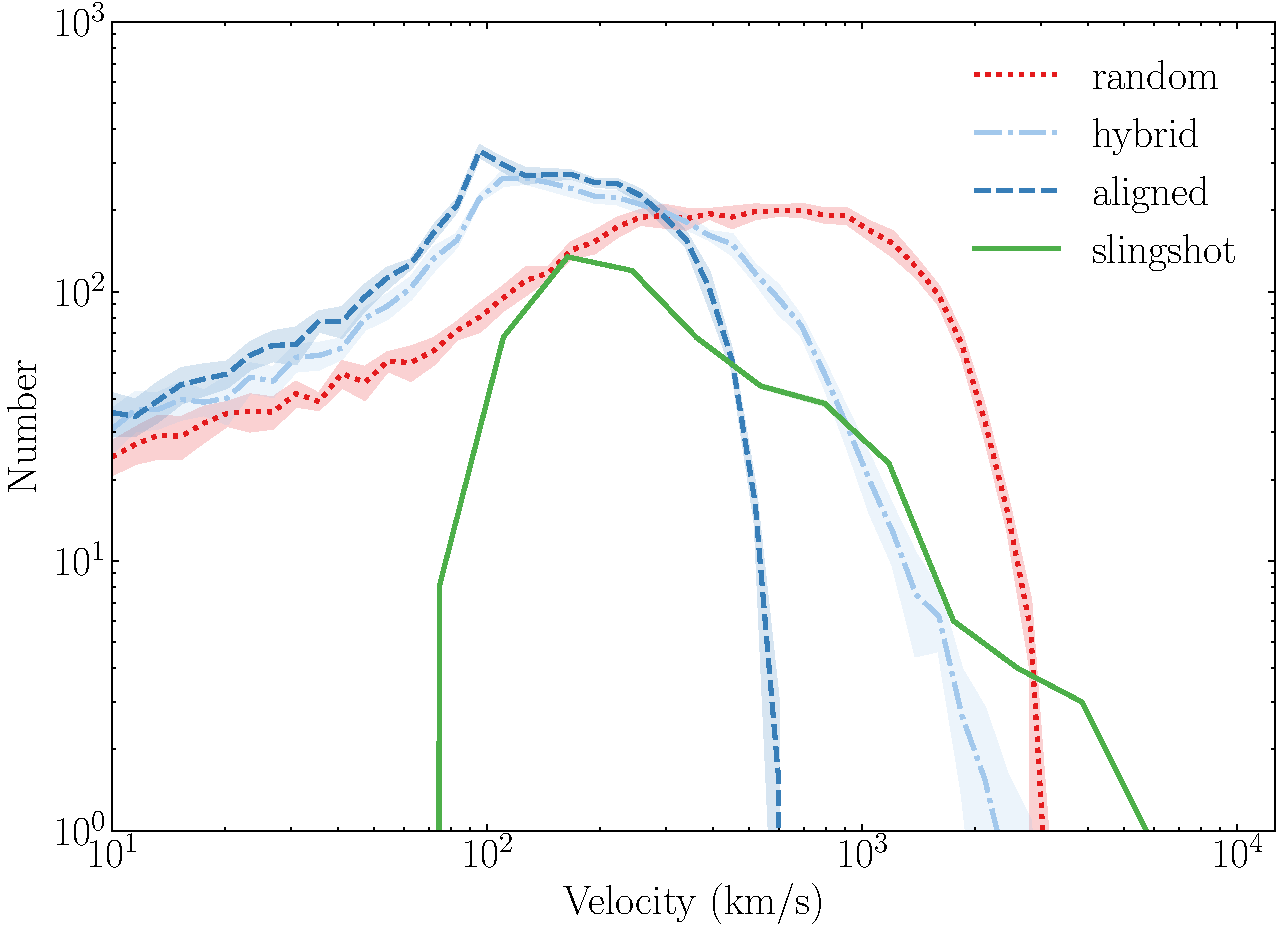
\includegraphics[scale=0.7]{fig/v-dist-for-all-kicks.pdf}
    \caption{Distribution of kick velocities of GW recoil for the different spin models: \texttt{random}, \texttt{aligned}, \texttt{hybrid}, and slingshot kicks averaged over all realizations.}
    \label{fig:kick-distributions-for-GW-recoil-and-slingshot}
\end{figure*}

\begin{table*}[!htb]
\centering
\resizebox{\textwidth}{!}
{\begin{tabular}{|l|l|l|l|l|l|}
\hline
\textbf{Kick type} & \textbf{Median $v_{\text{k}}$} & \textbf{Maximum $v_{\text{k}}$} & \textbf{\%$ v > 1000$ \kms} & \textbf{\%$v > 500$ \kms} & \textbf{\% of ejected} \\ \hline
GW recoil - \texttt{Random}            & 282.60 \kms                                 & 2750.22 \kms                 & $14.15 \pm 0.47$                    & $33.75 \pm 0.58$                     & $14.06 \pm 0.45$                     \\ \hline
GW recoil - \texttt{Hybrid}             & 131.59 \kms                                 & 3190.33 \kms                  & $1.23 \pm 0.20$                     & $9.10 \pm 0.39$                      & $1.78 \pm 0.20$                 \\ \hline
GW recoil - \texttt{Aligned}            & 106.38 \kms                                 & 610.68 \kms                  & 0                     & $0.54 \pm 0.13$                      & $0.23 \pm 0.06$                      \\ \hline
Slingshot kick         & 301.38 \kms                                  & 8149.61 \kms                  & $11.73 \pm 0.20$                    &   $26.65 \pm 0.27$                    & $8.73 \pm 0.13$                      \\ \hline
\end{tabular}
}
\caption{Statistics of the GW recoil kicks for the three different spin models and slingshot kicks. The values reported are averaged over 10 realizations of the spins.} 
\label{table:recoil-statistics} 
\end{table*}


We also asses the chances of kicks exceeding the host's central escape velocity, resulting in potential ejections. GW recoil kicks from \texttt{random} spins show the highest probability of ejections, with 14\% of kicks surpassing the escape velocity. Slingshot kicks follow, with 9\% exceeding this threshold. GW kicks from the \texttt{hybrid} spin model result in only 2\% of kicks exceeding escape velocities, while the \texttt{aligned} spin model contributes negligible ejections. These results are summarized in Table \ref{table:recoil-statistics}.

We now quantify the rates of ejections we see in our population due to the kicks produced from GW recoil and slingshot events. Recall that we are defining ejection for the case when $v_{\text{kick}} > v_{\text{esc}}$, where $v_{\text{esc}}$ is the central escape velocity of the host galaxy. The median escape speed in the total population is $\sim 1269$ \kms. We see from Figure \ref{fig:kick-distributions-for-GW-recoil-and-slingshot} that GW-recoil for random spins and slingshot kicks dominate above this range, suggesting they might be efficient in producing ejections. 

However, the total number of ejections from slingshot kicks is limited by the rarity of strong triple interactions. We examine the ejection rates within the population for GW recoil kicks across the \texttt{random}, \texttt{hybrid}, and \texttt{aligned} spin models, as well as for slingshot kicks. We compute the BH ejections through slingshot and gravitational wave recoil as discussed in Section \ref{sec: BH ejections} and calculate the new differential ejection rate using Equation \ref{eq: merger rate} where N now is the number of ejections. 

\begin{figure*}[!htb]
    \centering
    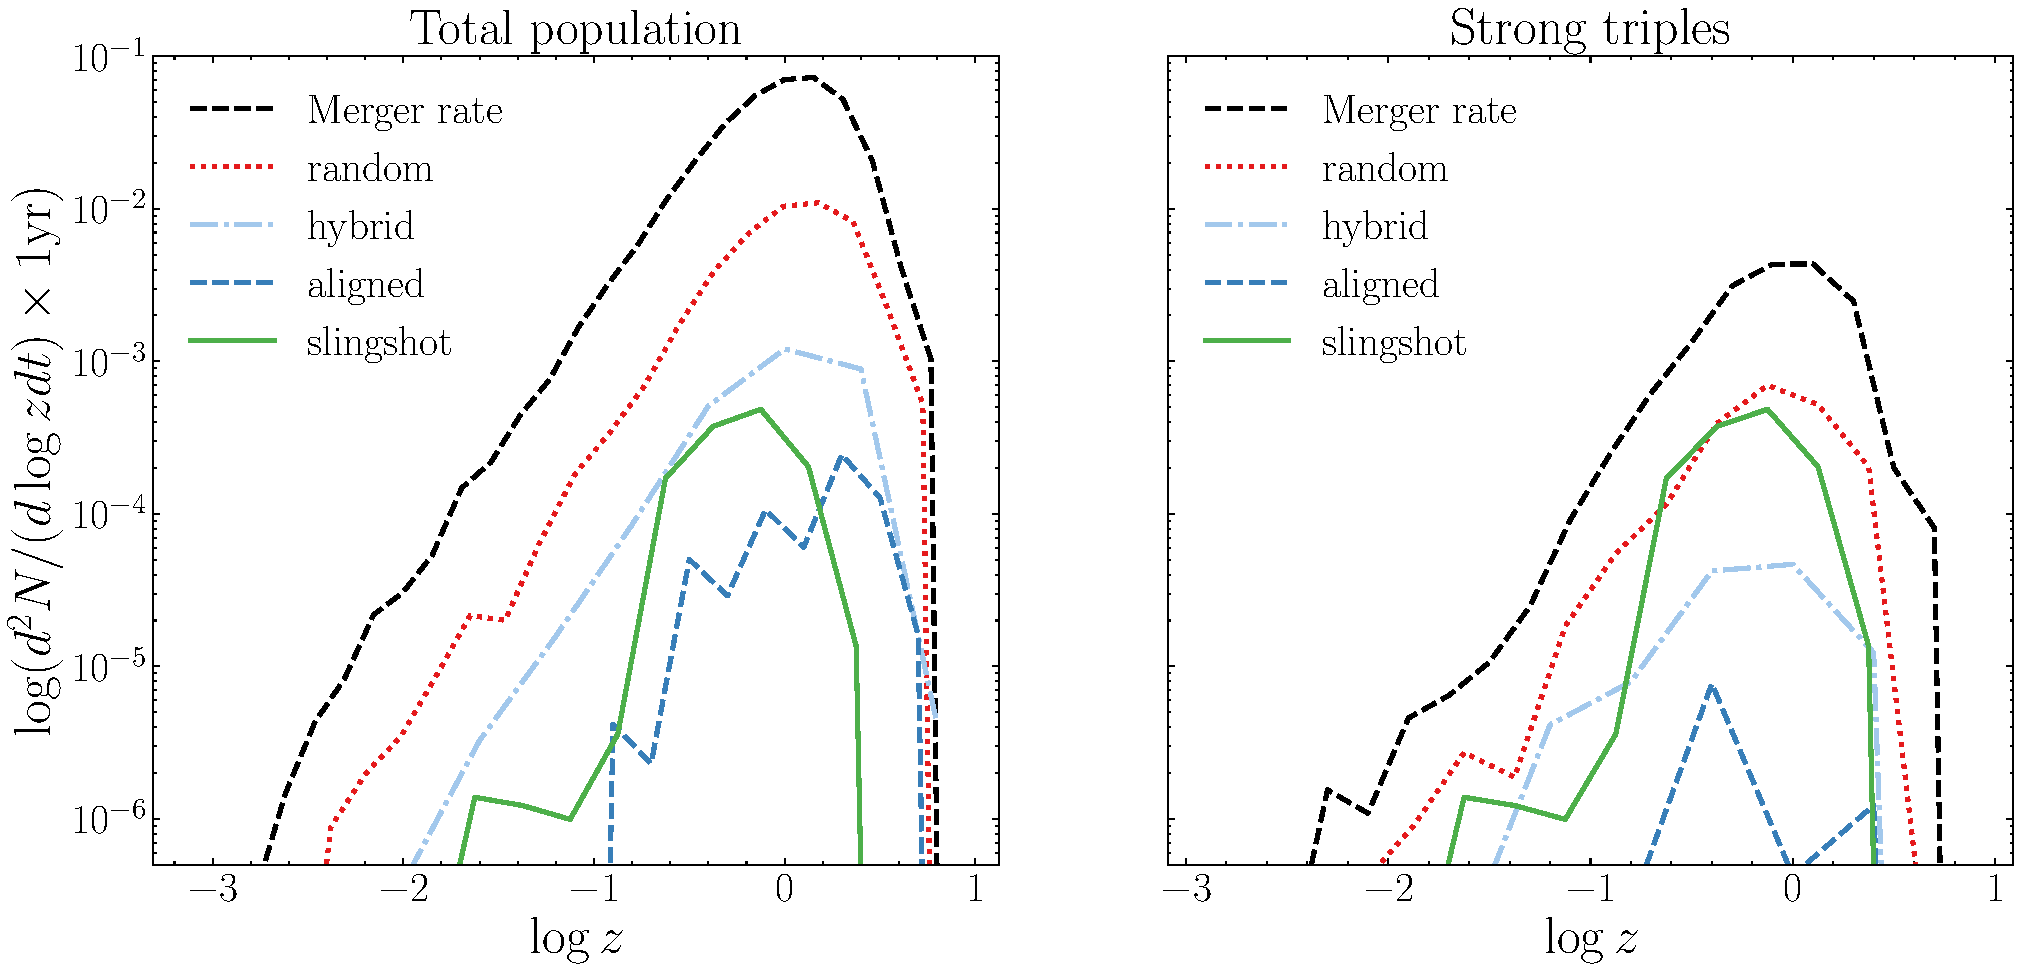
\includegraphics[scale=0.5]{fig/ejection_rates_all_and_triples_100.pdf}
    \caption{ Ejection rates (solid lines) vs merger rates over redshift in \textit{left}: the total population of binaries and triple systems and \textit{right}: only the strong triple systems.}
    \label{fig:escape-and-merger-rates-across-z}
\end{figure*}


In Figure \ref{fig:escape-and-merger-rates-across-z}, we plot the total ejection rates  from the random, hybrid, aligned GW kicks and slingshot kicks for the total population and the strong triples across all redshifts. For the total population, the ejection rates from random GW recoil kicks are approximately an order of magnitude lower than the merger rates (black dotted lines), while slingshot kicks are 2–3 orders of magnitude lower. However, within the strong triple subpopulation, the ejection rates from random GW recoil kicks and slingshot kicks are comparable in magnitude.

Within the strong triple subpopulation, slingshot kicks surpass GW recoil kicks from the hybrid spin model in ejection rates. In the total population, however, slingshot kicks produce ejection rates comparable only to GW recoil from the hybrid and aligned spin models. Across the total population, GW recoil from the random spin model result in the highest ejection rates overall. About $14 \%$ of mergers of binaries with random spins result in an ejection. Slingshot ejections make up to $\sim 1\%$ of the mergers, while the hybrid spin model is $\sim 2\%$ of the mergers. The aligned spin model produces almost no ejections with a $0.2 \%$ ejection fraction. The ejection fractions of GW recoil are in agreement with the values found in \cite{Blecha2016}. Within the strong triple subpopulation, it should be noted that ejections from random GW recoil kicks and slingshot kicks are both approximately $9 \%$ of the triple interaction outcomes. Thus, slingshot kicks are as relevant as GW kicks from random spins within the strong triple subpopulation.

Ejection rates tend to increase at higher redshifts, primarily due to the combination of lower escape velocities and elevated merger rates, which collectively lead to a greater number of ejections. For models such as aligned spins, the ejection rates from GW recoil kicks decrease significantly at lower redshifts. This behavior arises because aligned spin GW recoil kicks produce a maximum speed of 610 \kms, , which becomes insufficient to exceed the larger escape velocities typically found in galaxies at lower redshifts. In contrast, slingshot ejections can generate higher-velocity kicks, maintain the ability to produce ejections even at lower redshifts, where the escape speeds are higher.



MBH ejections will affect future mergers and the total merger rate. When an ejection occurs, the MBH escapes its host galaxy, preventing it from contributing to subsequent mergers. Our analysis shows that 5.6\% of mergers are prevented when considering slingshot ejections and GW recoil ejections in the random spin model. In contrast, only 1.6 \% of mergers are impacted by GW recoil ejections in the hybrid spin model, and just 0.2 \% are affected in the aligned spin model. This indicates that ejections have a minimal effect on the population unless the BH spins follow the random spin model. We also calculate the cumulative merger rate, removing the mergers that won't happen due to ejections. From GW recoil kick in random spins and slingshot kicks, the cumulative merger rate decreases from 0.402 yr$^{-1}$ to 0.387 yr$^{-1}$. The ejections from hybrid and aligned spin model produce negligible amount of difference in the merger rate.

\subsection{Future work}
\label{sec:future-work-dynamics}

My results show the importance of considering strong triple interactions in merging MBHs, as well as the relative contributions of gravitational slingshot and gravitational wave recoil to the overall MBH population.  One important caveat is that we treat strong triple interactions separately from the binary inspiral evolution in strong triples. In reality, hardening due to environmental effects in the binary and strong triple interactions likely occur simultaneously. Another important factor in strong triple systems is the eccentricity of binaries undergoing strong triple interactions. \cite{bonetti_post-newtonian_2018-1} observed that prompt mergers in triple MBH systems can drive binaries to high eccentricities. Therefore, we expect strong triple MBHs to have non-negligible eccentricities. This effect is also reflected in the characteristic strain spectrum, as shown in \cite{bonetti_post-newtonian_2018}, where the model including triple interactions deviates from the $f^{-2/3}$ power law. In future work, we plan to account for eccentricity in strong triples and develop a more self-consistent treatment of the inner binary evolution and strong triple interactions. Our approach will be applicable to any cosmological simulation, such as IllustrisTNG, to make robust predictions of the GWB for PTAs. 


Additionally, I plan to investigate these MBH dynamics in the early universe. I will characterize triple MBH interactions and include the effects of kicks in MBH binaries in the high redshift BRAHMA simulations \cite{bhowmick2024introducingbrahmasimulationsuite, bhowmick2024growthhighredshiftsupermassive} described in Section \ref{sec:cosmo-sim}. As mergers drive the growth of the low mass seeds in the early universe, multiple BH interactions are to be expected. Therefore, we can investigate triple MBH formation and their effects on the MBH merger rates observed by LISA. Additionally, recoil kicks are more significant at higher redshifts, affecting the growth of early BHs. Including recoiling BHs arising from both GW recoil and slingshot kicks could affect the merger rates predicted in BRAHMA and potentially increase the scatter in the MBH-galaxy correlations.


For the first project in this direction, I will use a simple time delay model to account for the merger timescale depending on the gas content of the merging environment similar to \cite{Blecha2016} and each binary will be evolved in isolation by incorporating these time delays. Triple MBHs will then be characterized following the procedure outline in Section \ref{sec:triple-outcomes} and Figure \ref{fig:trip-identify}. I will also investigate how host galaxy properties differ between systems hosting triple versus binary MBHs and also compare the triple MBH population across different BH seeding models. GW recoil and slingshot kicks will also be accounted for the triplets in the high-z universe following similar procedure as outline in . . Any MBH that receives a GW recoil or slingshot kick exceeding the host galaxy’s escape speed will be excluded from subsequent merger events. I will analyze how these ejections affect the assembly of MBHs in the early Universe by studying the MBH mass function and occupation fraction across redshifts. These properties will be compared across different BH seeding models and against a scenario with no ejections (\textbf{Project 1}). 

Building on the results of project 1, I will construct use the binary evolution model with all hardening mechanisms (section \ref{sec: insp-hardening-model}) and BH recoil effects for the second project. This model will numerically track the binary's evolution and will be applied to the simulations with different BH seeding models mentioned in \ref{sec:cosmo-sim} to determine their merger timescales accurately. Starting from the binary formation time in these simulations, I will evolve the binary separation using the dynamical-friction-based hardening \cite{Chandreshkar1943, Kelley_2018}, stellar-scattering \cite{Sesana_2006}, viscous drag from circumbinary disks \cite{HKM2009,Siwek2023,Siwek2024} and GW emission \cite{Peters_1963}. Additionally, I will track the evolution of the orbital eccentricity, starting from a fixed initial value, during stellar scattering \cite{Sesana_2008,Sesana_2015,Kelley_2018}, circumbinary disk \cite{Siwek2023,Siwek2024} and the GW-emission \cite{Peters_1963} phase.The binary evolution code \texttt{Holodeck} already incorporates most of these features.I will use this code with modifications to include triple interactions and the ability to adapt to the merger files from my cosmological simulation.

After evolving all binaries in isolation, successful triple MBH systems will then be detected by tracking the separation evolution of coexisting binaries ($a(t),t$), following \cite{sayeb_mbh_2023}. For cases where the intruder MBH approaches the galactic center, I will assume strong triple interactions and apply the sub-grid model from \cite{bonetti_post-newtonian_2018,bonetti_post-newtonian_2018-1}. These interactions may trigger a prompt merger (on timescales of $\sim 10^7$ yr) and impart a slingshot kick to the lightest MBH. If no prompt merger occurs, I will calculate the remaining binary separation \cite{volonteri_assembly_2003} and continue evolving it using the inspiral model. This binary hardening model, enhanced with triple interaction dynamics, will be applied to simulations with different BH seed models to predict LISA merger rates. The resulting merger rates will be compared with predictions from various semi-analytical models using heavy and light BH seeds (see Figure \ref{fig:SAM-merger-rates}).

\begin{figure}[!htb]
    \centering
    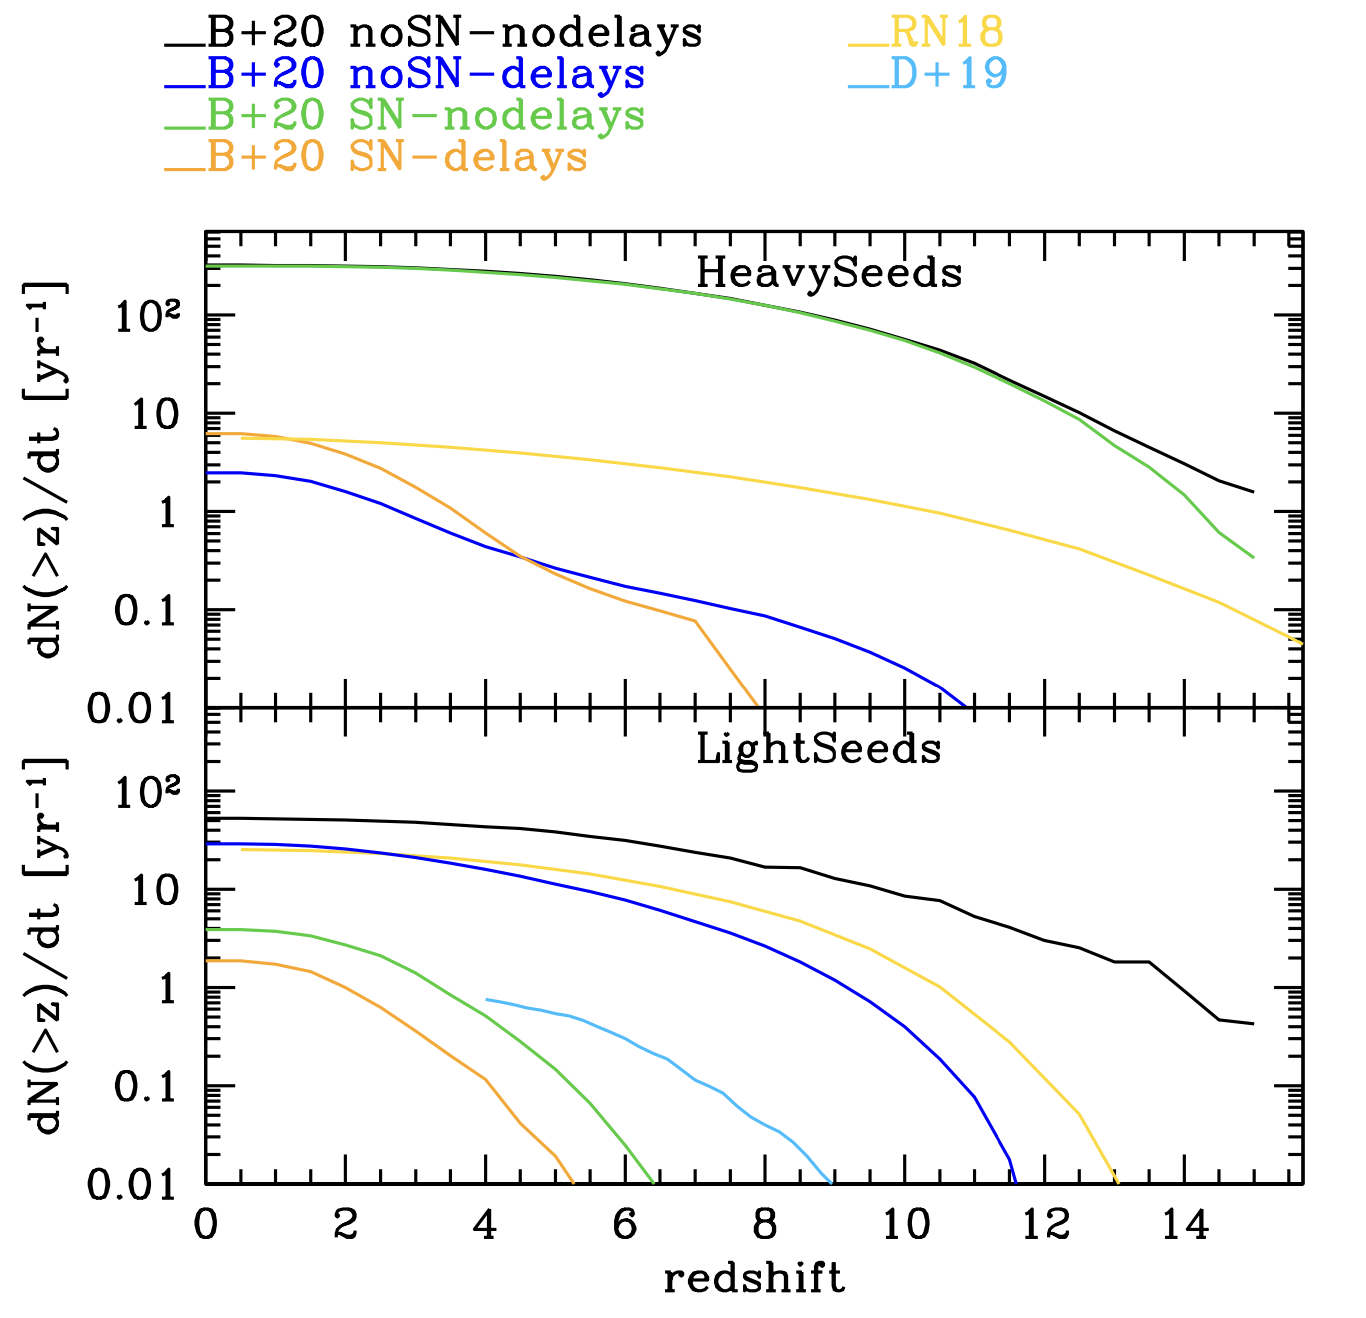
\includegraphics[width=0.7\linewidth]{fig/SAM_merger_rates_comparison.png}
    \caption{LISA Merger rates from different semi-analytical
models (SAMs) for heavy seeds (top panel) and light seeds
(bottom panel). The SAMs shown in this plot are from
[17, 68, 69] with different physical assumptions considered. The variations are a result of the uncertainty in the
modeling. The merger rates from the proposed work will
be compared with these predictions. Figure from \cite{Amaro_Seoane_2023}.}
    \label{fig:SAM-merger-rates}
\end{figure}

After each MBH merger, I will compute GW recoil with the spin orientation determined by comparing the alignment timescale to the inspiral timescale \citep{sayeb_massive_2021}. BHs receiving recoil or slingshot kicks exceeding the host galaxy’s escape speed will be removed from subsequent mergers. With BH ejections incorporated into the MBH dynamics model, I will explore various observational predictions with simulations using different seed models. Using the BH mass and galaxy stellar mass of spectroscopically confirmed JWST AGNs, I will compare the BH-host relation ($M_{\rm bh} - M_{*})$ with the MBH population across different seeding models. I will investigate how this relation evolves with redshift and compare it to the local scaling relation. The MBH mass function from simulations will be tested against local observational constraints, such as the bolometric quasar luminosity function such as from \citet{Shen_2020}. Additionally, I will compare the BH-host scaling relations and MBH mass function with results from other cosmological simulations, such as IllustrisTNG \citep{Springel_2017}. These findings will be published in a paper by the end of year 2. My MBH dynamics model can be easily adapted to other cosmological simulations, enabling a comprehensive study of the joint effects of BH seeding, growth, and dynamics (\textbf{Project 2}).



\section{Characterizing the host galaxies of MBH mergers}
\label{sec:host-galaxy-project}

As discussed previously in section \ref{sec:MBHB-evolution}, the host galaxy environment plays an important role in MBH binary evolution. Galaxy mergers can drive gas inflows, trigger star formation, and fuel AGN activity in the host environment. A key question, then, is: what are the defining characteristics of the host environments of merging MBHs? Do these enhancements persist till at the time of the MBH merger? If so, can we figure out definitive characteristics of host galaxies of GW sources and facilitate multimessenger observations? Our cosmological simulation suite enables us to explore these questions from the  low-redshift universe where MBH mergers maybe be observable through continuous GW  sources in PTAs—to the high-redshift regime, where LISA will detect MBH mergers.

\subsection{Analysis plan}

Using the cosmological simulations mentioned in Section \ref{sec:cosmo-sim}, we can identify the host subhalos where BH pairs form. This allows us to investigate the post-merger host galaxy environment, initially assuming that the BHs promptly merge after galaxy merger. In a subsequent project, we will also incorporate merger time delays using an MBH binary evolution model to track the descendant where the MBH merges.

The focus of the first project is to identify the sites where MBHs merge in the early universe and how they differ across the various seed models used in the BRAHMA simulation. To do this, we first identify merging galaxies that each host an MBH and then track their descendant in the next snapshot to establish the post-merger host galaxy. We will focus on major mergers defined by a mass ratio $q_{\rm merger} > 0.1$. To analyze the specific characteristics of these host galaxies, we will compare them with a control sample of non-interacting galaxies matched in redshift and stellar mass. Using BRAHMA, we can investigate if recent mergers result in AGN-enhancement, which is currently highly debated in the high-$z$ universe.

The matching in redshift and stellar mass follows methods similar to those in \citet{Ellison_2025, Hani_2020, Patton_2020}. We apply a minimum particle count threshold for dark matter and stars in our post-merger sample and filter only major mergers. For non-merging galaxies we also impose an additional criterion on their nearest companion. Following \citet{Patton_2020}, we define

\begin{equation} r_{\rm sep} = \frac{r}{R^{\rm gal}_{1/2} + R^{\rm comp}_{1/2}}, \end{equation}


where where $r$ is the separation of the non-merging galaxy from its
nearest companion, $R^{\rm gal}_{1/2}$ is the stellar half-mass
radius of the galaxy, and $R^{\rm comp}_{1/2}$ is the stellar
half-mass radius of the nearest companion. We exclude those galaxies with $r_{\rm sep} \leq 2$ to ensure that only isolated galaxies are included in the control sample.

To create the control sample from non-interacting galaxies we use the following 
algorithm: for each post-merger host, we identify the closest matching non-interacting galaxy in redshift, $z$ and stellar mass, $M_{\star}$. We then perform a Kolmogorov-Smirnov(KS) test to assess the statistical similarity of the two distributions. The matching is repeated iteratively without replacement until either $\rm p < 0.99$ or at least ten control galaxies are assigned per post-merger host. This provides us with a sample of matched controls per merging host. This matching algorithm is first tested on the TNG-50 simulation and the results are discussed in the next section. 

After obtaining a sample of host and control we aim to examine key properties such as specific  star formation rate and BH accretion. By examining these characteristics across different BH seed models in BRAHMA, we aim to investigate where any differences in the host environments where BHs most often merge in the early Universe. We expect to see the differences between the merging environment to be most dramatic at the high-z universe before subsequent mergers erase this information. This comparison will yield key predictions for early MBH growth and provide insights relevant for future LISA observations (\textbf{Project 3}).

For the second project in this focus area, we will apply the BH binary inspiral model discussed in \ref{sec: insp-hardening-model} to trace the host galaxies of MBH mergers detectable via gravitational waves. For this work, we will use the TNG-50 simulation, which tracks MBH evolution up to low-redshifts to the epoch of GW observations through PTAs. For each identified galaxy merger, we apply the postprocessing MBH inspiral models to calculate the delay time associated with the MBH merger. After which, we trace the descendant of the merging galaxy down the merger tree to find the galaxy close to the snapshot that corresponds to the computed merger time. Additionally galaxies with stalled MBH binaries at $z=0$ will be identified and classified into those that are could be potential GW sources identifiable by PTAs.  We can compare the  non interacting galaxies matched in $z$ and $M_{\star}$ to the GW hosts and identify key properties that distinguish the hosts from the non interacting galaxies. Moreover, we can study the evolution of key galaxy properties of the GW host after galaxy merger until the BH coalescence (\textbf{Project 4}). 

\subsection{Preliminary results}
   
\begin{figure}[!htb]
    \centering
    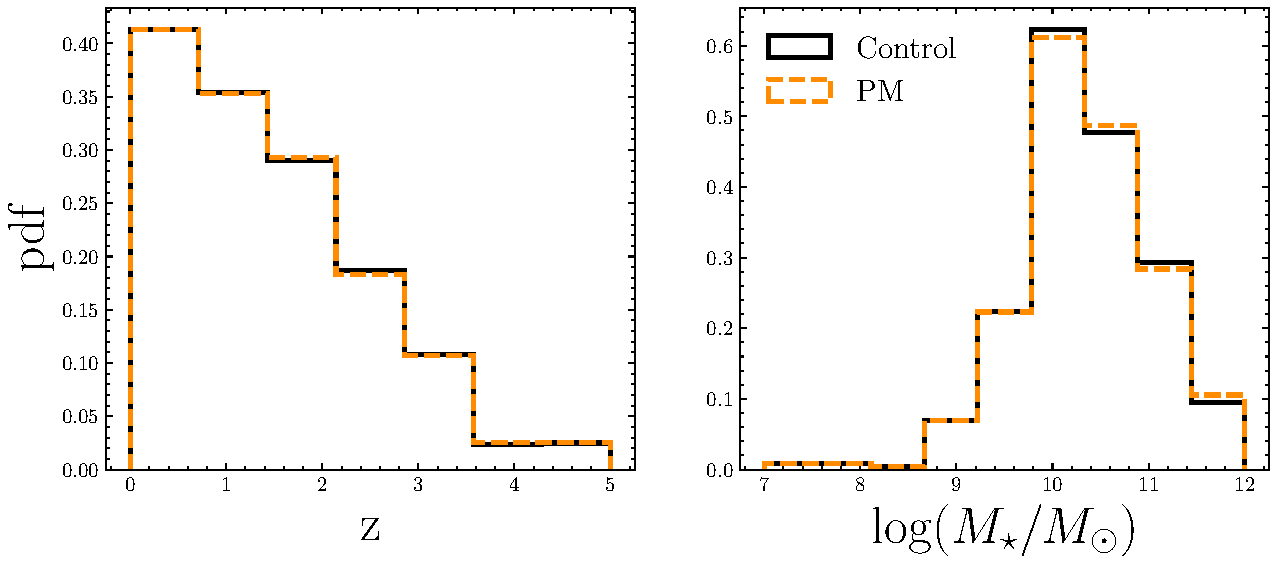
\includegraphics[width=0.8\linewidth]{fig/control-pm-z-Mstar-match.pdf}
    \caption{The distribution of redshift (left) and stellar mass $M_{\star}$(right) for the post-meger samples and control samples created for TNG50. }
    \label{fig:control-matching}
\end{figure}

We begin by demonstrating the approach of analyzing host galaxies of MBH mergers using the TNG-50 simulation. From the simulation, we extract galaxy mergers each containing a BH and satisfying a minimum particle cut of 100 DM particles, 100 gas particles, and 100 stellar particles. This selection yields a total of 467 such mergers in TNG-50. We then filter the sample to include only major galaxy mergers ($\mu>0.1$), resulting in 444 mergers.  For each of these major mergers, we construct control samples from non-interacting galaxies via the matching method described in the previous section. This gives us 10 control galaxies matched in redshift and stellar mass for each post-merger sample. The match between the control samples and post-merger galaxies is visualized in Figure \ref{fig:control-matching}. The redshift is matched within a tolerance of $\pm 0.5\%$  and $\pm 0.03$ dex for $M_{\star}$ on average. 

\begin{figure}
    \centering
    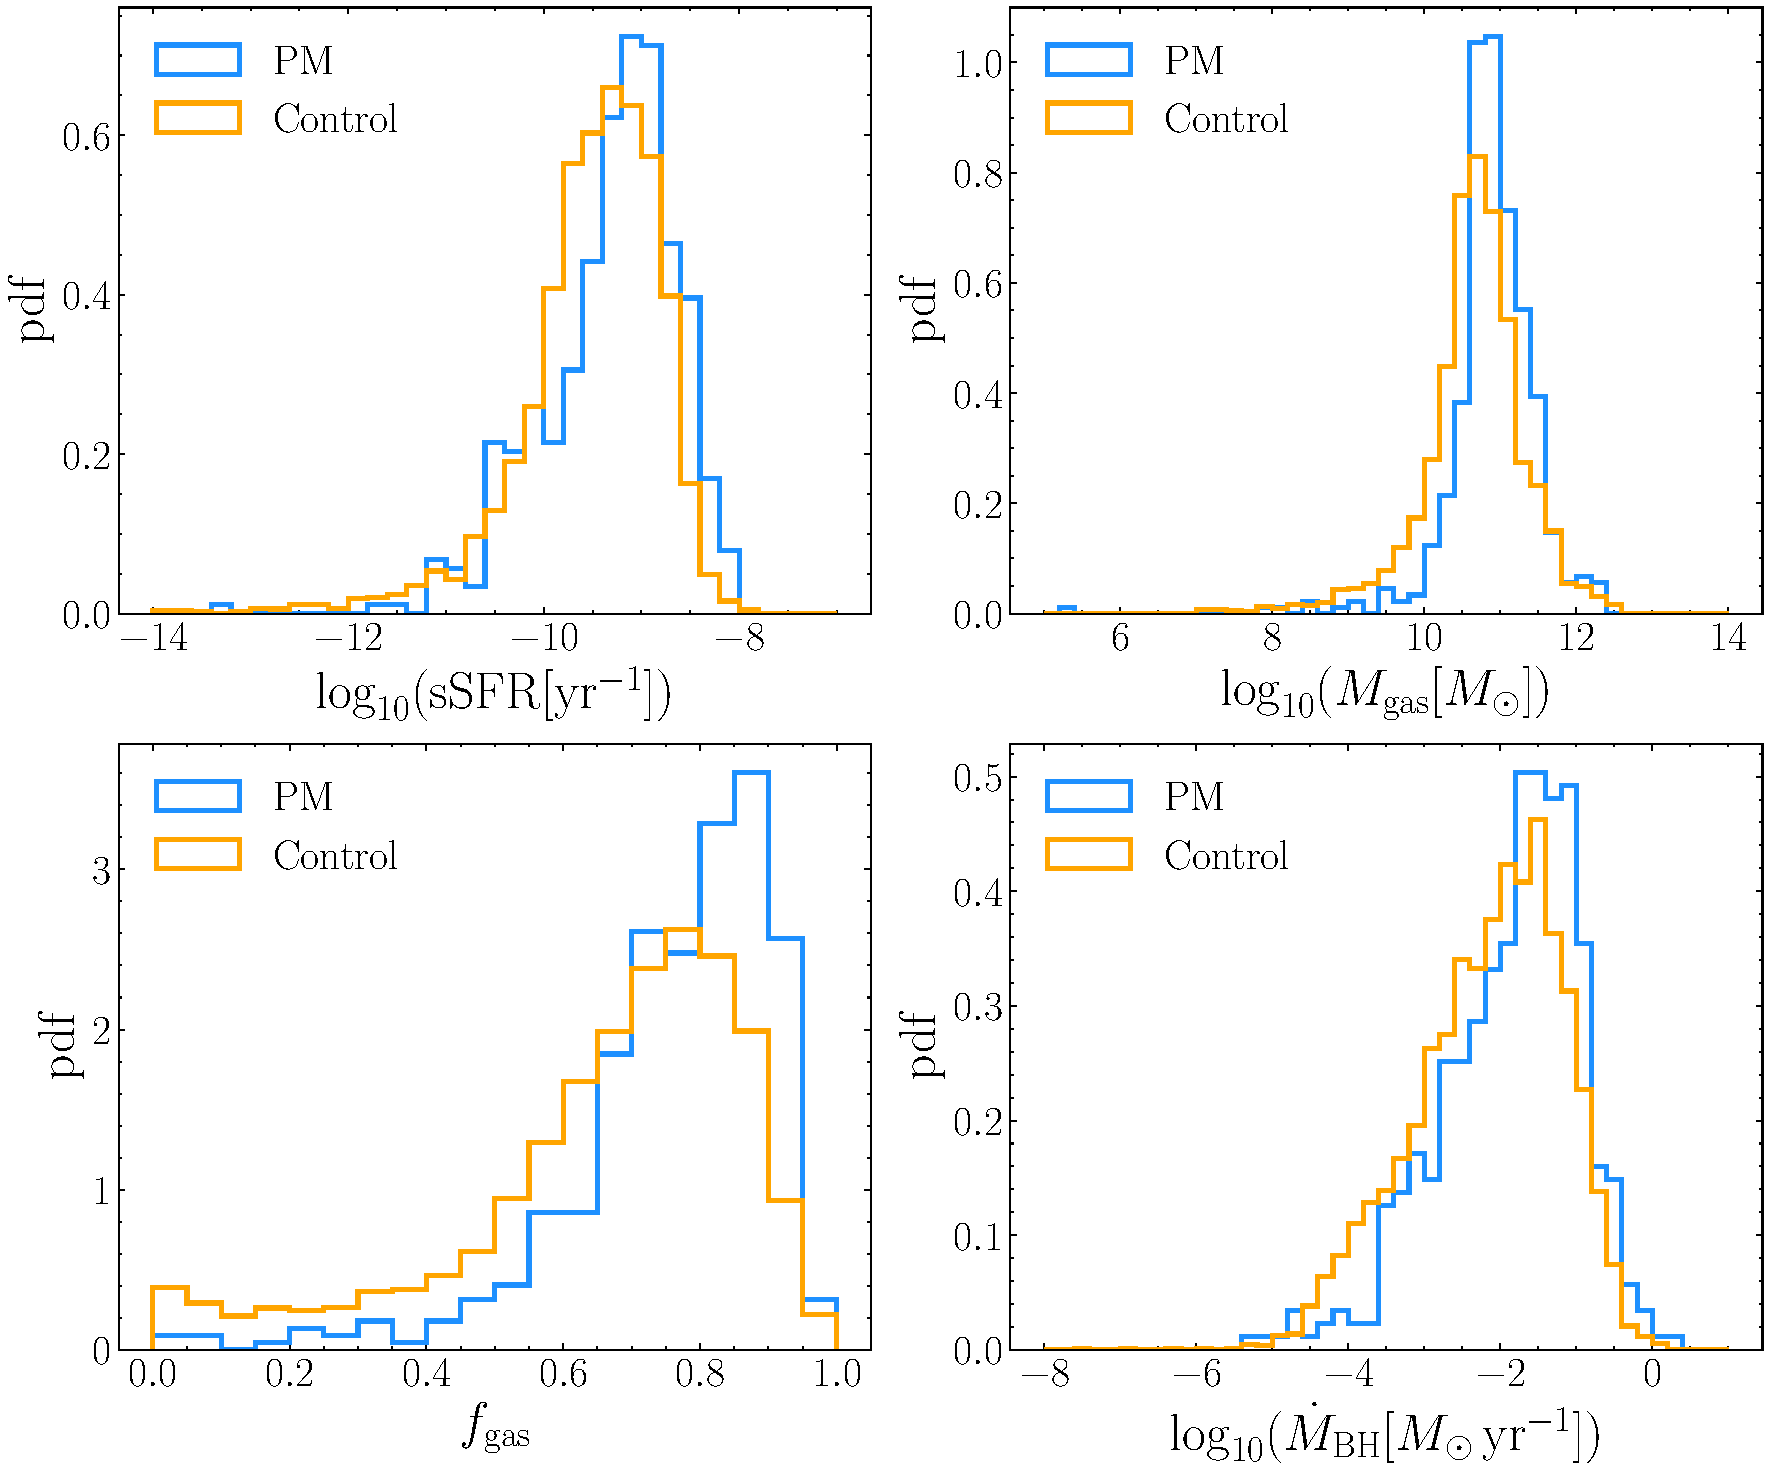
\includegraphics[width=0.7\linewidth]{fig/mergers_vs_control_properties_hist.pdf}
    \caption{Distribution of i) specific star formation rate, ii) gas-mass, iii) gas fraction and iv) black hole accretion among the post merger and control samples.}
    \label{fig:hist-merger-control-comparison}
\end{figure}

Several works have demonstrated the impact of galaxy mergers on host characteristics, including morphological disturbances \citep{DeGraf_2021,Patton2016}, enhanced SFR \citep{Ellison_2008,Ellison_2013} , AGN fractions \citep{Satyapal_2014,Ellison_2011} and gas fractions \citep{Ellison_2018}.To investigate similar enhancements in our sample, we compare the properties of post-merger galaxies to their control counterparts. Figure \ref{fig:hist-merger-control-comparison} shows the distribution of specific star formation rate (sSFR), gas content ($M_{\rm gas}$) and black hole accretion rates ($\dot{M}_{\rm BH}$) for the post merger samples and the control samples. We find that post mergers have an average black hole accretion rate of $\dot{M}^{\rm PM}_{\rm BH} = 6.013 \times 10^{-2} M_{\odot} \rm yr^{-1}$ and the controls have an average of $\dot{M}^{\rm control}_{\rm BH} = 3.538 \times 10^{-2}M_{\odot} \rm yr^{-1}$. The enhancement of post merger black hole accretion is $\sim$ 1.7 and matches with the findings reported in \cite{Byrne_Mamahit_2022}. They also find that the SMBH accretion enhancement can last upto $\sim 2$ Gyr, whereas the SFR enhancement that only lasts $\sim 500$ Myr. 

\begin{figure}[htp]
    \centering
    \begin{minipage}{0.45\textwidth}
        \centering
        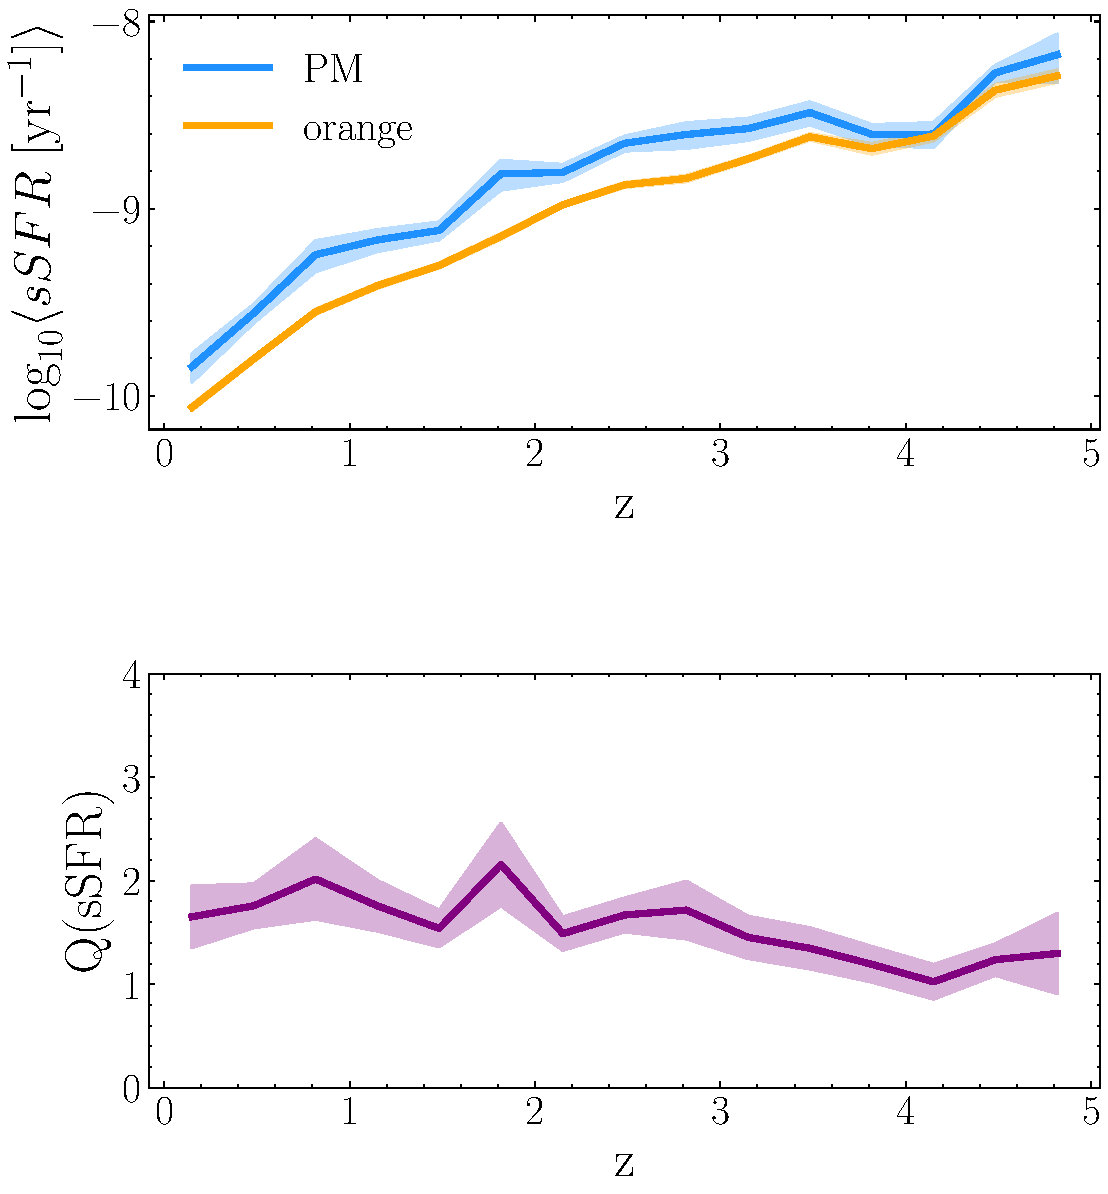
\includegraphics[width=1\linewidth]{fig/sSFR_z_evolution_merger_vs_control.pdf}
        %\caption{Caption for sSFR evolution}
        \label{fig:sSFR_evolution}
    \end{minipage}
    \hspace{0.05\textwidth}  % Adjust the space between the two subfigures
    \begin{minipage}{0.45\textwidth}
        \centering
        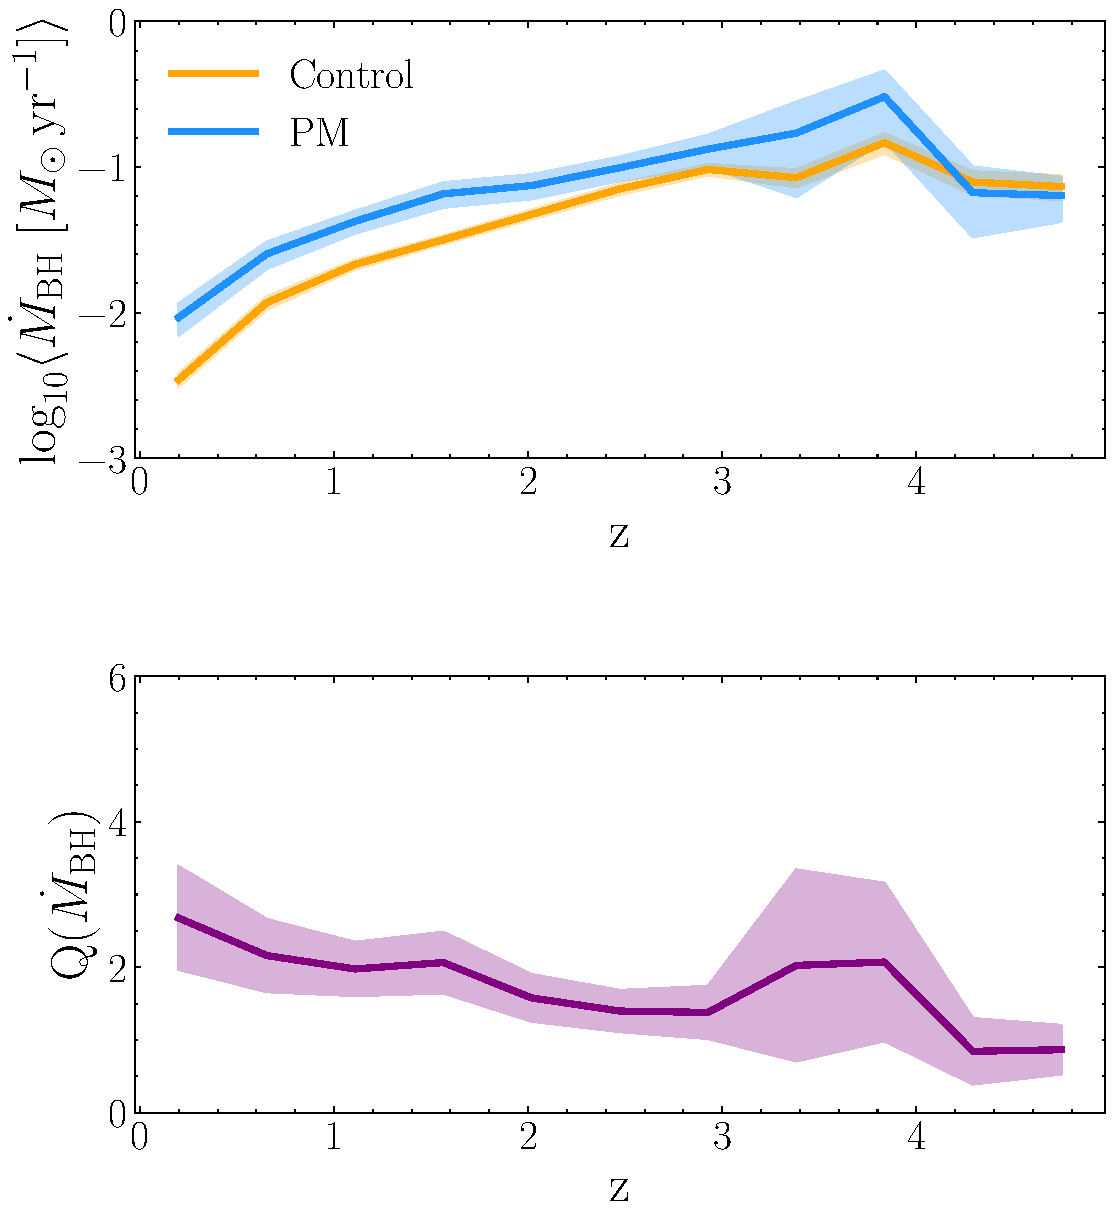
\includegraphics[width=1\linewidth]{fig/mdot_z_evolution_merger_vs_control.pdf}
        %\caption{Caption for Mdot evolution}
        \label{fig:mdot_evolution}
    \end{minipage}
    \caption{Redshift evolution of specific star formation rate (left, top-panel) and black hole accretion rate (right, top panel) of the post-merger and control samples. The bottom panels show the enhancement of sSFR and $\dot{M}_{\rm BH}$ with redshift. The average enhancement in sSFR is $\rm Q(sSFR) = 1.553 \pm 0.241$ and$\dot{M}_{\rm BH}$ is $\rm Q(\dot{M}_{\rm BH}) = 1.732 \pm 0.558$   }
    \label{fig:sSFR-Mdot-redshift-evolution}
\end{figure}

We also find an average sSFR enhancement in post-mergers $\sim 1.6$ times more than the control galaxies. This enhancement is slightly lower than what was reported in \cite{Hani_2020}. This is likely due to differences in the control sample selection criteria. Their work additionally required to have no past mergers within the last $< 2$ Gyr ago. Since do not apply this restriction on the controls, ours criteria is less stringent, potentially including galaxies that recently underwent mergers, thereby having some enhancement in SFR. We do not observe a significant enhancement in the gas mass or gas fraction between the post-merger and control samples. We see only an enhancement of $\sim 1.2$ and $\sim  1.3$ for $f_{\rm gas}$ and $M_{\rm gas}$ respectively. It should also be noted that studies like \cite{Byrne_Mamahit_2022} match their controls to post-mergers in gas mass as well and they find that the accretion rate enhancement is dependent on the gas mass of the merging galaxy. 

For the next steps, we aim to apply additional constraints on the control sample and explore which property matching criteria are necessary to study enhancements in mergers, particularly to inform the control samples for BRAHMA. 

For the first project in this area, we aim to apply the matching method to the BRAHMA simulation to create a sample of hosts of BH mergers and control samples of non interacting subhalos, consider a prompt merger scenario for the BHs. A key goal of this project is to compare across different BH seeding models available to characterize where BHs merge in the early universe. We will also be able to look for how the various properties such as black hole accretion rate enhancement in the high redshift universe something that hasn't been explored in previous studies with cosmological simulations. 

Secondly, in our TNG300 analysis we plan on applying the postprocessing MBHB model described in \ref{sec:future-work-dynamics}. We will follow the binary along the merger tree and identify the closest snapshot at which the binary has merged. The descendant subhalo in this snapshot will be considered as the host galaxy of an MBH merger. This approach will allow us to build a population of GW host sources and characterizes their properties. We will perform a control sample analysis with non merging properties and identify any distinct properties of the GW host sources. Moreover, we will also look for binaries that remains stalled at $z=0$ at sub-pc separations that could be potenital GW sources detectable by PTAs. 




\section{Timeline}
\label{sec:timeline}
The following is a rough timeline of the activities planned for future works of the projects described in this  report. 

\begin{figure}[!htb]
    \centering
    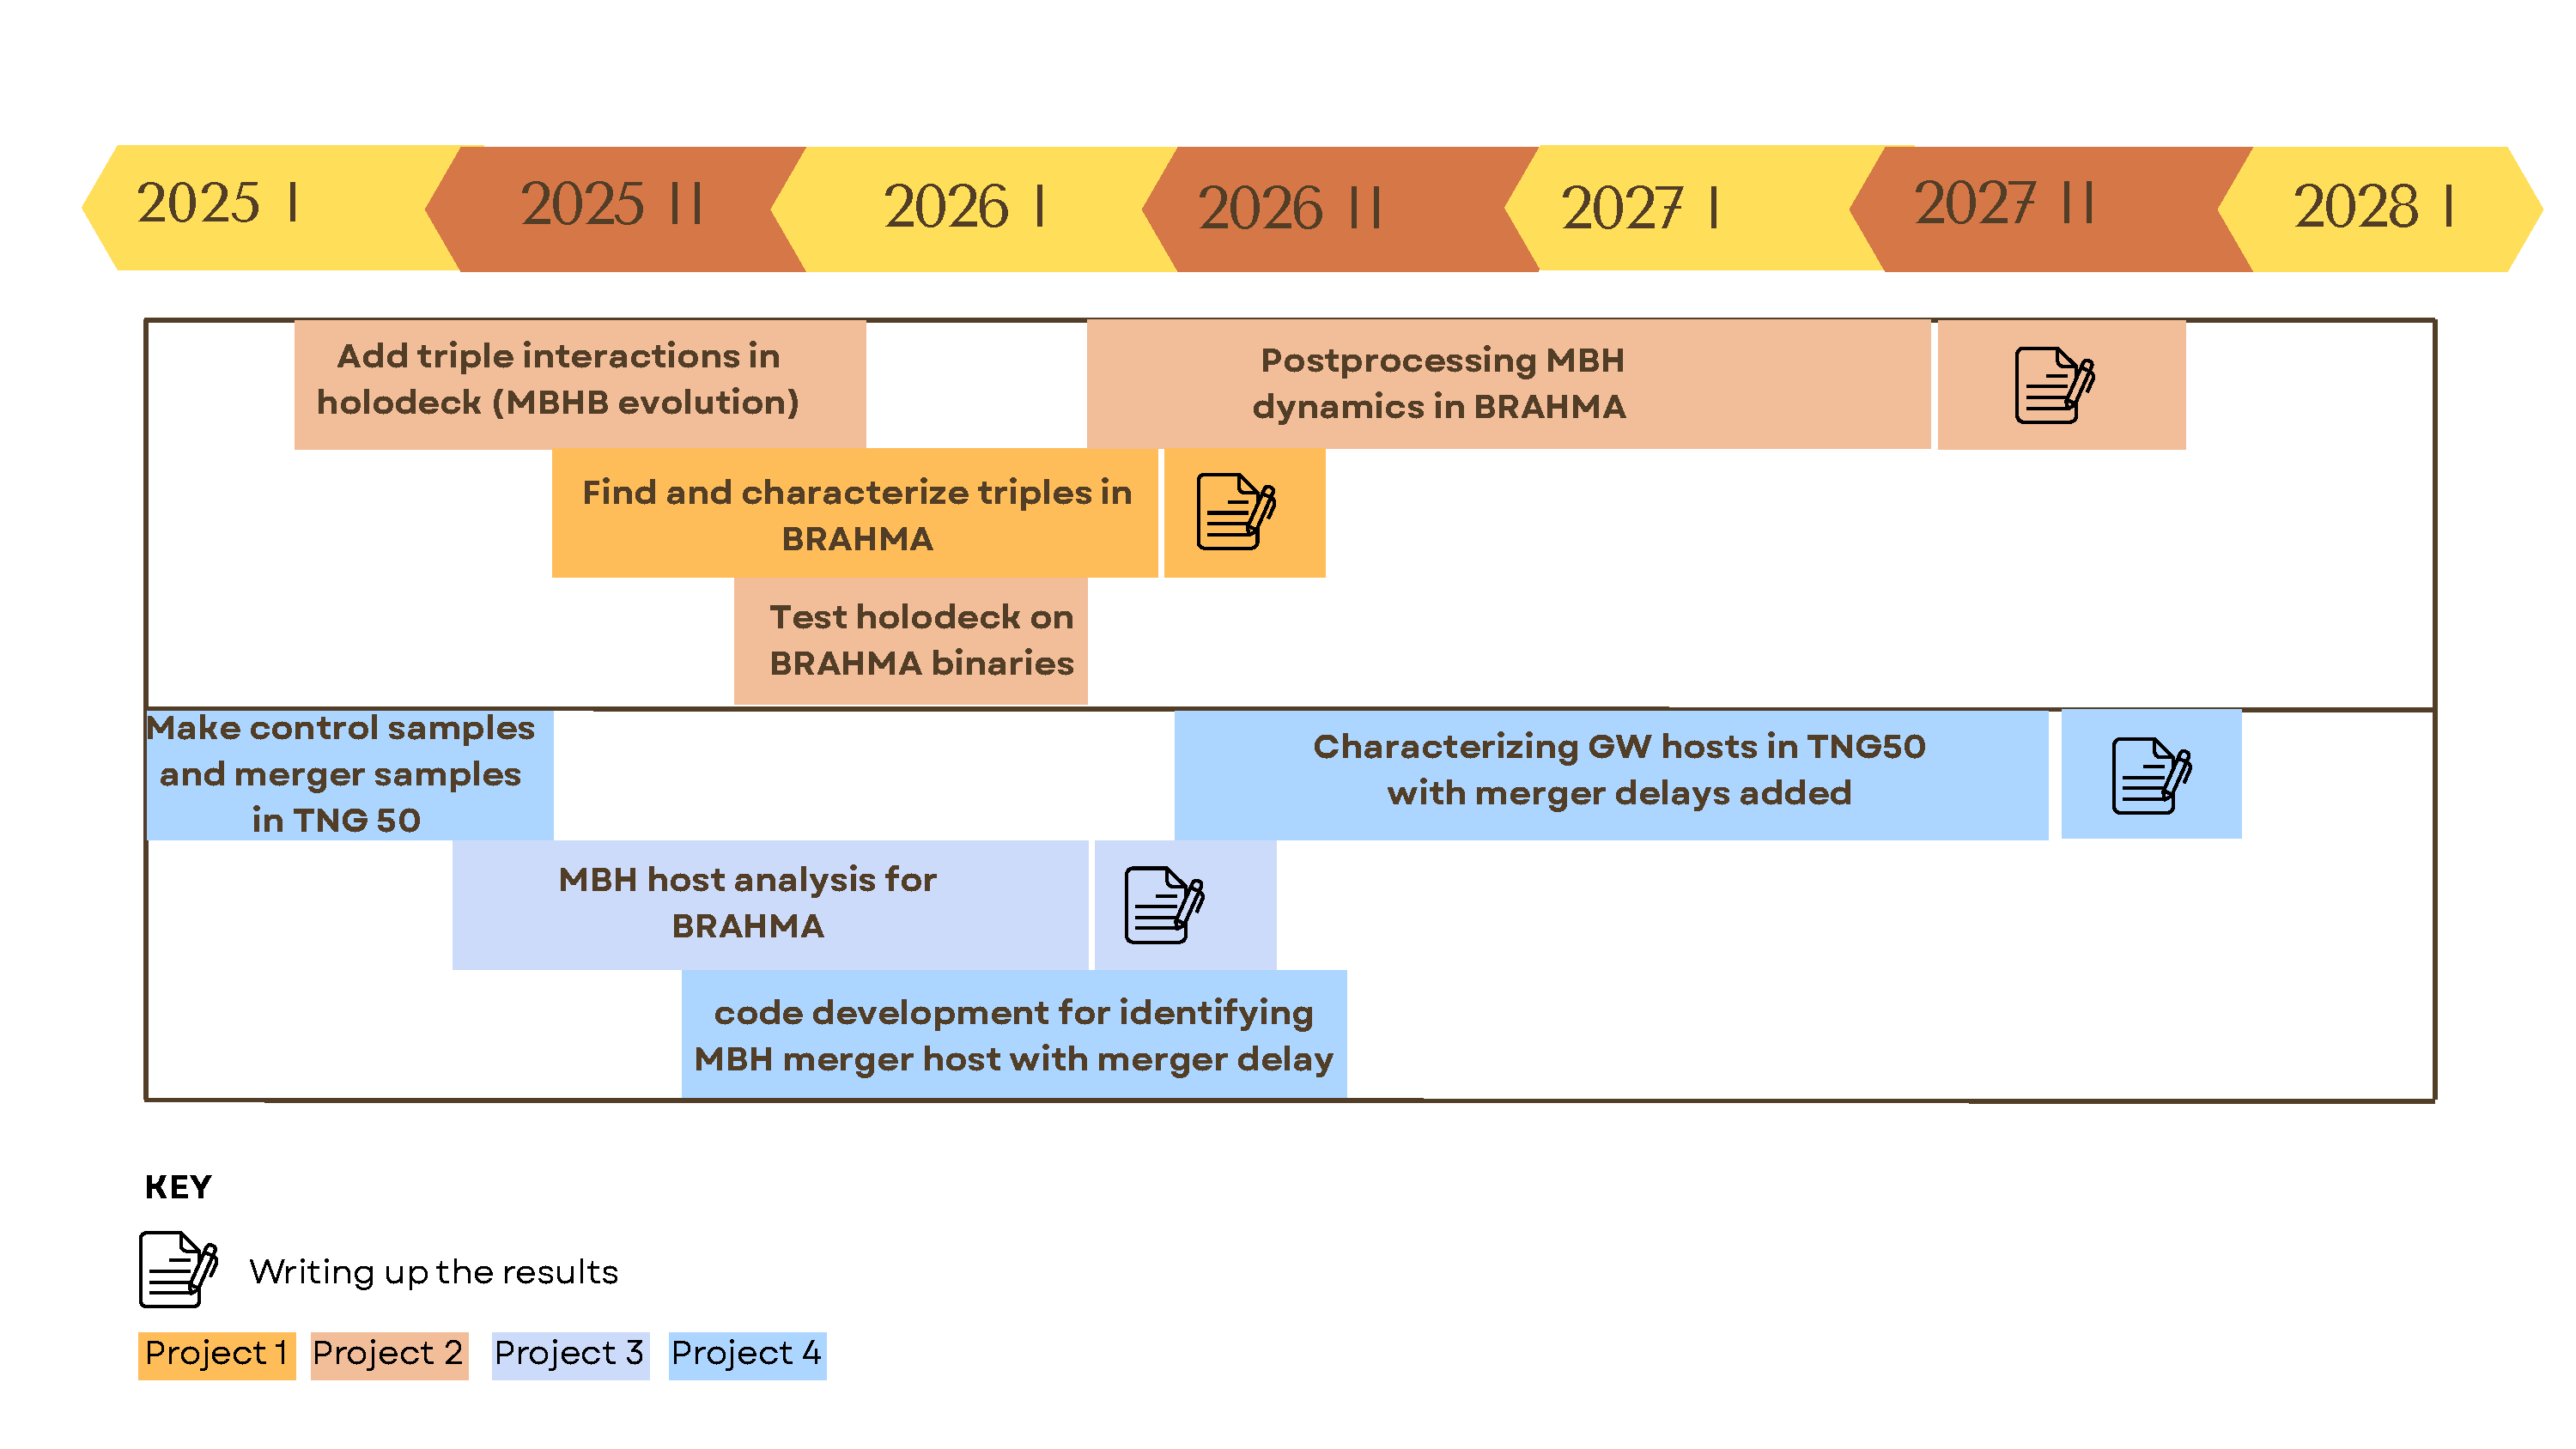
\includegraphics[scale=0.34]{fig/Graduate timeline.pdf}
    \caption{Timeline of the planned work}
    \label{fig:timeline}
\end{figure}

\begin{itemize}
    \item \textbf{2025-2026}
    \begin{enumerate}
        \item The results of the triple outcomes from Illustris is ready for submission soon.
        \item Development of code to create control samples matched to mergers for both TNG-50 and BRAHMA (Project 3 and 4).
        \item Work to include triple interactions in \texttt{Holodeck} to have a postprocessing MBHB evolution code ready for evolving binaries from simulations. (Project 2)
        \item Extract the details of MBH merger hosts in BRAHMA and apply the code developed for matching the mergers to control samples of non-mergers (Project 3)
        \item Find the triple MBH systems in the high redshift universe using BRAHMA and study the impact of black hole kicks. (Project 1)
        
    \end{enumerate}
    \item \textbf{2026-2027}
    \begin{enumerate}
        \item Write up results of triple interactions in BRAHMA. (Project 1)
        \item Apply \texttt{Holodeck} in TNG-50 binaries and calculate delay. Develop code to identify descendent hosts of MBH mergers. (Project 4)
        \item Perform the MBH merger host analysis in BRAHMA and write up the results for publication. (Project 3)
        \item Apply the post-processing \texttt{Holodeck} model in BRAHMA binaries.(Project 2) 
    \end{enumerate}
    \item \textbf{2027-2028}
    \begin{enumerate}
        \item Analyze the mergers in the BRAHMA sims. Also add BH kicks and ejections in postprocessing.
        \item Analyze the population of GW host sources from TNG-50 after applying merger delays. Write up the results for publication. (Project 4)
        \item Write up the results of the post-processed MBH mergers in BRAHMA for publication. (Project 2)
    \end{enumerate}
\end{itemize}

% % Acknowledgments
% \phantomsection
% \addcontentsline{toc}{section}{Acknowledgments}
% \section*{Acknowledgments}
\label{sec:ack}

\lipsum[6]

% \newpage

% References

\phantomsection
\addcontentsline{toc}{section}{References}
\bibliographystyle{unsrtnat}
\bibliography{bib/refer, bib/mypub}
\newpage

% % Paper records
% \phantomsection
% \addcontentsline{toc}{section}{Appendix: Publications}
% \section*{Appendix: Publications}
\label{sec:pub}
\setcounter{NAT@ctr}{0}

% Replace this example with your records.

% Published
\nocitemypub{example1_published, example2_published}
\bibliographystylemypub{unsrtnat}
\bibliographymypub{bib/mypub}

% Under Review
\nocitereview{example3_review}
\bibliographystylereview{unsrtnat}
\bibliographyreview{bib/mypub}

% In Preparation
\nociteprepare{example4_prepare}
\bibliographystyleprepare{unsrtnat}
\bibliographyprepare{bib/mypub}


\end{document}